% wedoc.tex V1.0, 17 June 2010

\documentclass[times]{weauth}

\usepackage{moreverb}

\usepackage[colorlinks,bookmarksopen,bookmarksnumbered,citecolor=red,urlcolor=red]{hyperref}

%% Code syntax highlighting

\usepackage{listings}
\usepackage{color}

\definecolor{mygreen}{rgb}{0,0.6,0}
\definecolor{mygray}{rgb}{0.5,0.5,0.5}
\definecolor{mymauve}{rgb}{0.58,0,0.82}
\definecolor{mylightgray}{rgb}{0.95,0.95,0.95}

\lstset{frame=single,
    % language=C++,
    aboveskip=3mm,
    belowskip=3mm,
    showstringspaces=false,
    columns=flexible,
    basicstyle=\ttfamily,
    numbers=none,
    numberstyle=\tiny\color{mygray},
    keywordstyle=\bfseries\color{blue!40!black},
    commentstyle=\color{gray},
    stringstyle=\color{mygreen},
    % otherkeywords={for,if,else},
    breaklines=true,
    breakatwhitespace=true,
    tabsize=4,
    escapeinside={\%*}{*)},
    keepspaces=true,
    captionpos=b,
    backgroundcolor=\color{mylightgray}
}

\graphicspath{{figures/}}

\newcommand\BibTeX{{\rmfamily B\kern-.05em \textsc{i\kern-.025em b}\kern-.08em
T\kern-.1667em\lower.7ex\hbox{E}\kern-.125emX}}

\def\volumeyear{2016}

\begin{document}

\runningheads{P.~Bachant \emph{et al.}}{Actuator line modeling of vertical-axis
turbines}

\articletype{RESEARCH ARTICLE}

\title{Actuator line modeling of vertical-axis turbines}

\author{P.~Bachant\textsuperscript{1}, A.~Goude\textsuperscript{2}, and
M.~Wosnik\textsuperscript{1}}

\address{\textsuperscript{1}Center for Ocean Renewable Energy,
University of New Hampshire, 24
Colovos Rd., Durham, NH, 03824, USA \\
\textsuperscript{2}Department of Engineering Sciences,
Division of Electricity, Uppsala University, Uppsala 751 21, Sweden}

\corraddr{M.~Wosnik, Chase Ocean Engineering Laboratory, University of New
Hampshire, 24 Colovos Rd., Durham, NH, 03824, USA. \\
E-mail: martin.wosnik@unh.edu}

\begin{abstract}
    To bridge the gap between high and low fidelity numerical modeling tools for
    vertical-axis (or cross-flow) turbines (VATs or CFTs), an actuator line
    model (ALM) was developed and validated for both a high and a medium
    solidity vertical-axis turbine at turbine diameter Reynolds numbers $Re_D
    \sim 10^6$. The ALM is a hybridization of classical blade element theory
    with Navier--Stokes based flow models, and in this study both
    $k$--$\epsilon$ Reynolds-averaged Navier--Stokes (RANS) and Smagorinsky
    large eddy simulation (LES) turbulence models were tested. The RANS models
    were able to be run on coarse grids while still providing good convergence
    behavior in terms of the mean power coefficient, and also approximately four
    orders of magnitude reduction in computational expense compared with 3-D
    blade-resolved RANS simulations. Submodels for dynamic stall, end effects,
    added mass, and flow curvature were implemented, resulting in reasonable
    performance predictions for the high solidity rotor, more discrepancies for
    the medium solidity rotor, and overprediction for both cases at high tip
    speed ratio. The wake results showed that the ALM was able to capture some
    of the important flow features that contribute to VAT's relatively fast wake
    recovery---a large improvement over the conventional actuator disk model.
    The mean flow field was better realized with the LES, which still
    represented a computational savings of two orders of magnitude compared with
    3-D blade-resolved RANS, though vortex breakdown and subsequent turbulence
    generation appeared to be underpredicted, which necessitates further
    investigation of optimal subgrid scale modeling.
\end{abstract}

\keywords{wind turbine; VAWT; cross-flow turbine; blade element theory; dynamic
stall; lifting line}

\maketitle


\section{Introduction}

Vertical-axis (cross-flow) turbines (VATs or CFTs) were the subject of
significant research and development in the 1970s through the 1990s by groups
like Sandia National Labs in the US~\cite{Sutherland2012} and the National
Research Council of Canada~\cite{Para2002}. Despite minor commercial success for
large scale onshore wind applications, vertical-axis turbines were virtually
abandoned in favor of horizontal-axis (or axial-flow) turbines, as they
generally are more efficient and don't encounter the high levels of fatigue
loading that VATs do. Today, however, there is renewed interest in VATs for
marine hydrokinetic (MHK) applications~\cite{ORPC2012}, offshore floating wind
farms~\cite{Paulsen2011, Sandia2012, Dodd2014}, and smaller scale, tightly
spaced wind farms~\cite{Dabiri2011, Kinzel2012}, thanks to their relatively
faster wake recovery.

The mean near-wake structure of vertical-axis turbine has been shown to be
largely dominated by the effects of tip vortex shedding, which induces levels of
recovery due to vertical advection significantly larger than those from
turbulent fluctuations~\cite{Bachant2015-JoT}---an effect not seen in HAT wakes.
As interest shifts to designing and analyzing arrays of VATs, it is necessary to
determine the effectiveness of various numerical modeling techniques to
replicate VAT near-wake dynamics, such that wake recovery is accurately
predicted, leading to accurate assessment of optimal array spacing.

Reynolds-averaged Navier--Stokes (RANS) turbulence models computed on 3-D
body-fitted (blade-resolved) grids can do a good job predicting the mean
performance and near-wake structure of a VAT, though their effectiveness depends
on the turbulence model applied~\cite{Bachant2016-BR-CFD}. However, 3-D
blade-resolved RANS presents a huge computational expense---on the order of
1,000 CPU hours per simulated second with contemporary hardware---since it must
resolve fine details of the blade boundary layers, which will preclude its use
for array analysis until the availability of computing power increases
sufficiently. It is therefore necessary to explore simpler models that can
predict the turbine loading and flow field with acceptable fidelity, but that
are economical enough to not require high performance computing, at least for
individual devices.

Very fast solution times can be obtained with blade element momentum (BEM)
models, such as the double multiple streamtube (DMST) approached developed by
Paraschivoiu~\cite{Para1988}. However, their poor performance for high loading
or streamwise induction factors, common for rotors with high
solidity~\cite{Joo2015} $Nc/R$ (and/or chord-to-radius ratio $c/R$), where $N$
is the number of blades, $c$ is the chord length, and $R$ is the maximum rotor
radius, makes them less attractive, particular for marine hydrokinetic
applications where rotors of the same size will encounter approximately an order
of magnitude higher torque compared to wind turbines. Their description of the
flow field is very crude as well, simply computing the momentum contained within
discretized streamtubes, which cannot resolve any of the complicated flow
structures shed by the rotor, limiting their applicability for array analysis.

Blade element based vortex line methods, e.g., \cite{Strickland1981,
Murray2011}, can be solved with reasonable computational effort when coupled
with potential flow models---ranging from an expense close to BEM up to that of
2-D blade-resolved CFD. The cost is a function of the number of vortex elements,
which for free vortex methods may increase at each time step, slowing down the
calculation as it marches forward in time, unless there is an additional model
for vortex diffusion. Potential flow vortex methods can resolve more flow
details than BEM. However, since the flow is governed by the Laplace equation,
nonlinear effects such as the turbulent transport will not be included, which we
have determined in experiments to be the same order of magnitude as the mean
vertical advection.

It is therefore desirable to retain a Navier--Stokes description of the flow
field and use an actuator-type model for parameterizing the turbine loading,
which dramatically drives down computational expense by removing the need for
complicated meshes with many fine cells to resolve the boundary layers near the
blade surfaces. As shown in \cite{Bachant2015-JoT}, the conventional uniform
actuator disk is not a good candidate for a cross-flow turbine wake generator,
never mind the fact that it does not typically compute performance predictions.
There are then two actuator methods that use blade element theory to compute
blade loading and therefore generate a wake that more closely resembles that of
an actual turbine. These are the actuator cylinder or swept-surface model (ASSM)
and the actuator line model (ALM). The ASSM solves for the average blade loading
along its path and applies this as a constant body force term in the momentum
equation. The ALM takes a similar approach but is an unsteady method, resolving
the blade element locations in time.

The ALM, originally developed by Sorensen and Shen \cite{Sorensen2002}, has
become popular for modeling axial-flow or horizontal-axis turbines, and has been
shown in blind tests to be competitive with blade-resolved
CFD~\cite{Krogstad2013, Pierella2014}. The ALM combined with large eddy
simulation has become the state-of-the-art for modeling entire wind
farms~\cite{Archer2013, Churchfield2012, Sorensen2015, Fleming2013,
Fleming2014}. Like other blade element techniques, the effectiveness of the ALM
for AFTs is in part due to the quasi-steady nature of the flow in the blade
reference frame, and the relatively rare occurrence of stall. Note that a
similar method can be used with the Navier--Stokes equations in
vorticity--velocity form~\cite{Scheurich2011b}, which may be more efficient when
vorticity is confined to a relatively small fraction of the domain, e.g., for a
standalone turbine with a uniform laminar inflow.

The ASSM and ALM were implemented to model a very low Reynolds number 2-D
cross-flow turbine experiment in a flume using large eddy simulation
(LES)~\cite{Shamsoddin2014}. Performance predictions for this case were not
reported, but the ALM was shown to be more effective at postdicting the wake
characteristics measured in the experiments by Brochier et
al.~\cite{Brochier1986}.

It is therefore proposed that an actuator line model may be the optimal
combination of high-fidelity flow modeling that includes performance
predictions, but with reduced computational expense. Here we have developed an
ALM for cross-flow turbines inside both RANS and LES simulations, implemented as
an extension for the OpenFOAM open-source CFD library. This model was validated
against experimental data for both a high \cite{Bachant2015-JoT} and a medium
\cite{Bachant2016-RM2-paper} solidity vertical-axis turbine.


\section{Turbines}

Two turbines were modeled: the high solidity ($c/R=0.28$) UNH Reference
Vertical-Axis Turbine (UNH-RVAT) and the medium solidity ($c/R=0.07$--$0.12$) US
Department of Energy/Sandia National Labs Reference Model 2 (RM2) cross-flow
turbine (at 1:6 scale), both of which are shown in Figure~\ref{fig:turbines}.
Both rotors are of similar geometric size ($\sim 1$ m) and are constructed from
symmetrical NACA foils mounted at mid-chord and mid-span.

Open datasets for the performance and near-wake dynamics of the UNH-RVAT and
RM2, available from \cite{Bachant2014-RVAT-baseline,Bachant2016-RVAT-Re-dep} and
\cite{Bachant2016-RM2-data}, respectively. have been acquired in the UNH towing
tank at Reynolds numbers based on turbine diameter $Re_D = 10^6$. Analysis of
these datasets showed that turbine performance and near-wake characteristics
were nearly Reynolds number independent in this
regime~\cite{Bachant2016-Energies,Bachant2016-RM2-paper}.

\begin{figure}
    \centering

    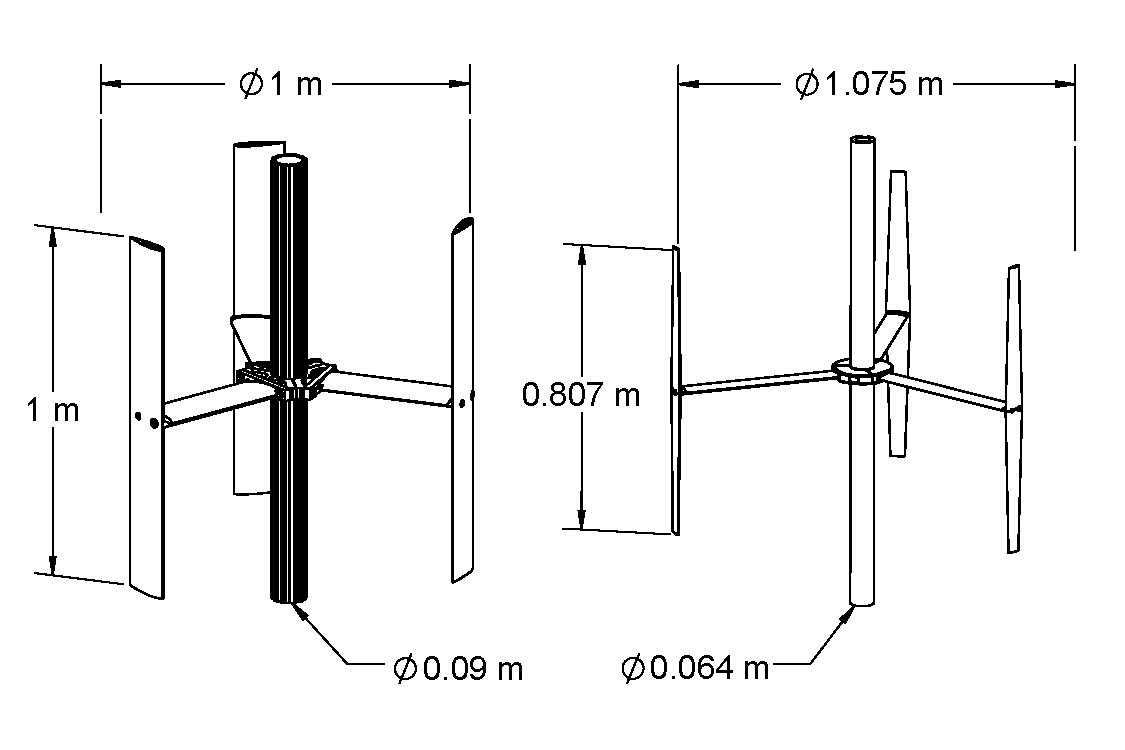
\includegraphics[width=0.6\textwidth]{turbines}

    \caption{Drawings of the turbines modeled in this study: the UNH-RVAT (left)
    and DOE/SNL RM2 (right).}

    \label{fig:turbines}
\end{figure}


\section{Theory}

The actuator line model is based on the classical blade element theory combined
with a Navier--Stokes description of the flow field. The ALM treats turbine
blades as lines of blade elements, for which 2-D profile lift and drag
coefficients are given. For each blade element, relative flow velocity and angle
of attack are computed by adding the vectors of relative blade motion and the
local fluid velocity, a diagram of which is shown in Figure~\ref{fig:vectors}.

\begin{figure}
    \centering

    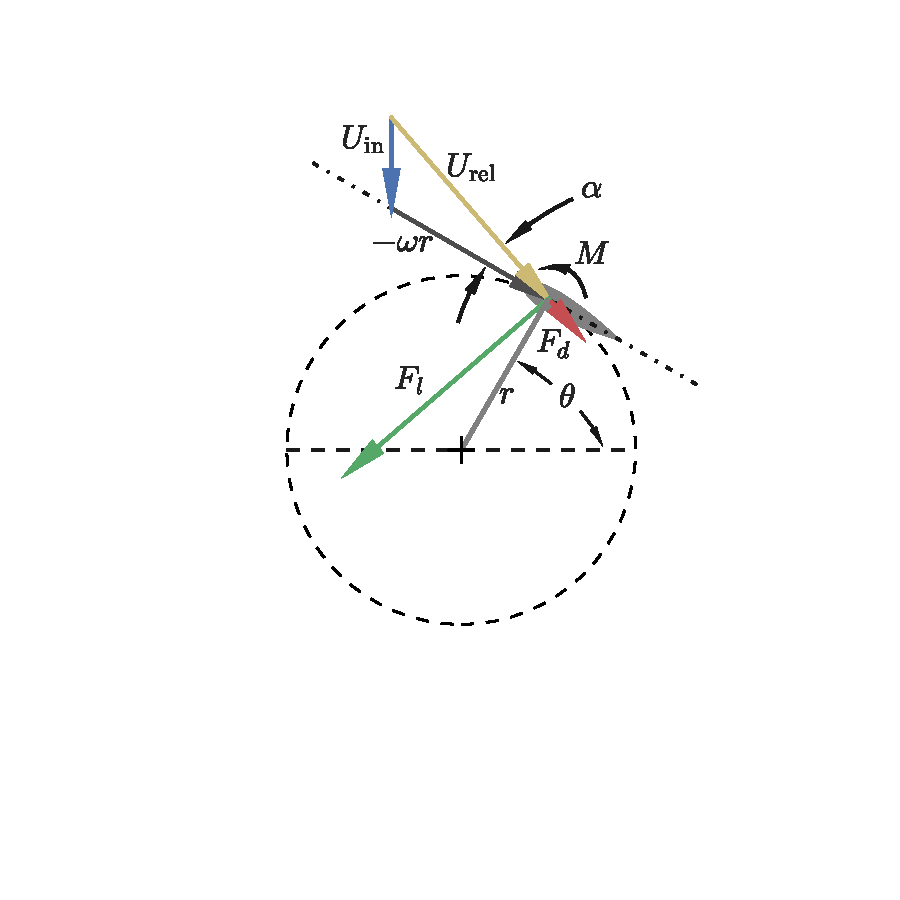
\includegraphics[clip, trim=1in 1.5in 1in 0.5in,
    width=0.4\textwidth]{figures/CFT-vectors_cft-vectors}

    \caption{Vector diagram of velocity and forcing on a cross-flow turbine
        blade element. Note that the free stream velocity $U_\infty$ is from top to
        bottom (identical to $U_in$ for purely geometric calculations), the blade
        chord (dash-dotted line) is coincident with the tangential velocity (i.e.,
        zero preset pitch, which would offset the geometric angle of attack
        $\alpha$), and the drag vector is magnified by a factor of two
        (approximately, relative to the lift vector) to enhance visibility.}

    \label{fig:vectors}
\end{figure}

The kinematics of a CFT are parameterized by the tip speed ratio $\lambda =
\omega R/U_\infty$, where $\omega$ is the shaft's angular velocity, $R$ is the
maximum rotor radius, and $U_\infty$ is the free stream velocity. Using only
geometric considerations---that is, ignoring the effect of the rotor forcing and
assuming the inflow velocity to be equal to that of the free stream---the
geometric angle of attack $\alpha$ and relative velocity magnitude
$|\vec{U}_{\mathrm{rel}}|$ can be calculated as a function of the rotor
azimuthal angle $\theta$, which is plotted for various tip speed ratios in
Figure~\ref{fig:geom-alpha-urel}.

\begin{figure}
    \centering

    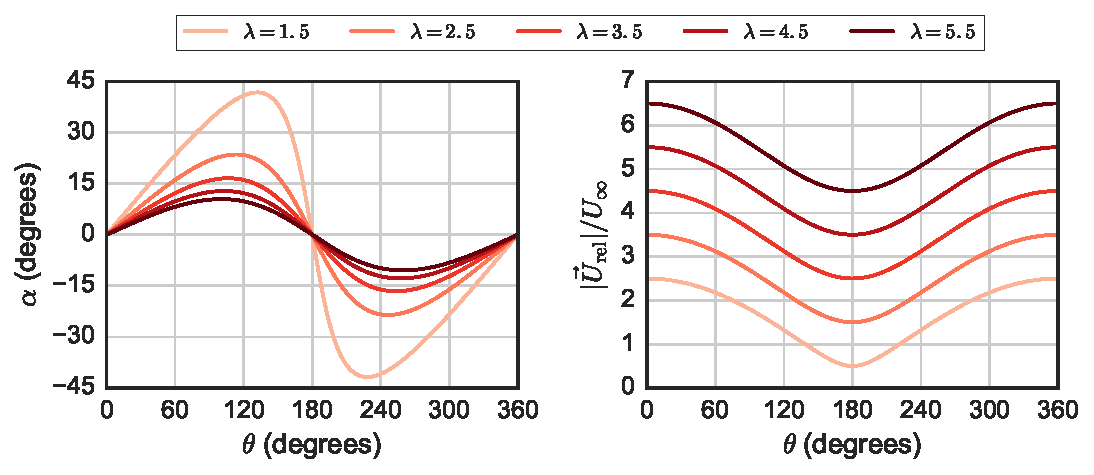
\includegraphics[width=0.75\textwidth]{CFT-vectors_alpha_deg_urel_geom}

    \caption{Geometric angle of attack (left) and relative velocity (right)
        versus azimuthal angle at various tip speed ratios.}

    \label{fig:geom-alpha-urel}
\end{figure}

Inspecting Figure~\ref{fig:geom-alpha-urel}, it is apparent that CFTs are
inherently unsteady machines, encountering large amplitude and rapid
oscillations in angle of attack, often exceeding the rotor blades' static stall
angles in typical operation. The unsteadiness can be characterized by a reduced
frequency~\cite{Leishman2006}
\begin{equation}
    k = \frac{\omega c}{2 U_\infty},
\end{equation}
which assumes the free stream velocity is constant. Unsteady effects begin to
become significant for $k > 0.05$, and can become dominant for $k \ge 0.2$.

For a VAT or CFT reduced frequency can be reformulated in terms of the tip speed
ratio as
\begin{equation}
    k = \frac{\lambda c}{2R},
\end{equation}
which is then also a function of solidity or chord-to-radius ratio $c/R$. As an
example, a large scale, relatively low solidity Darrieus wind turbine such as
the Sandia 34 m diameter Test Bed, with an equatorial blade chord of 0.91 m
\cite{Murray2011}, a reduced frequency $k=0.16$ is encountered based solely on
angle of attack oscillations at $\lambda=6$. For a smaller scale CFT, e.g., with
$c/R = 0.25$, operating at $\lambda = 2$, the reduced frequency is 0.25. It
follows that unsteady effects will be significant for cross-flow turbines even
in the absence of nonlinear effects such as stall.

Assuming unsteady effects can be appropriately modeled, the blade element lift force, drag forces, and pitching moment are calculated as
\begin{equation}
    F_l = \frac{1}{2} \rho A_\mathrm{elem} C_l |\vec{U}_\mathrm{rel}|^2,
\end{equation}
\begin{equation}
    F_d = \frac{1}{2} \rho A_\mathrm{elem} C_d |\vec{U}_\mathrm{rel}|^2,
\end{equation}
\begin{equation}
    M = \frac{1}{2} \rho A_\mathrm{elem} c C_m |\vec{U}_\mathrm{rel}|^2,
\end{equation}
respectively, where $\rho$ is the fluid density, $A_\mathrm{elem}$ is the blade
element planform area (span $\times$ chord), $\vec{U}_\mathrm{rel}$ is the local
relative velocity projected onto the plane of the element profile cross-section
(i.e., the spanwise component is neglected), and $C_l$, $C_d$, and $C_m$ are the
sectional lift, drag, and pitching moment coefficients, respectively, which are
linearly interpolated from a table per the local angle of attack. The forces are
then projected onto the rotor coordinate system to calculate torque, overall
drag, etc. Forces from the turbine shaft and blade support struts are computed
in a similar way. After the force on the actuator lines from the flow is
computed, it is then added to the Navier--Stokes equations as a body force or
momentum source (per unit density, assuming incompressible flow):
\begin{equation}
    \frac{\mathrm{D} \vec{u}}{\mathrm{D} t} = - \frac{1}{\rho} \nabla p + \nu
    \nabla^2 \vec{u} + F_\mathrm{turbine}.
\end{equation}


\section{Blade element discretization}

In the ALM, a turbine is a collection of actuator lines, which themselves are
collections of actuator line elements (ALEs). The position of each ALE is a
point in space indicating its quarter-chord location. The element is further
defined by its chord direction vector, chord length, span direction vector, span
length, and velocity vector.

An actuator line is created from defined geometry points, between which ALE
parameters are interpolated linearly. This way, an actuator line can be defined
by fewer geometry points than element locations. For example, an AL with
straight planform boundaries---e.g. a straight or tapered wing---only needs two
geometry points to be fully defined. Figure~\ref{fig:AL-geom} shows and example
schematic of a tapered actuator line with three geometry points at the
half-chord locations and six total elements. Note that the middle geometry point
is technically redundant, but is shown for illustrative purposes. For actuator
lines that represent bluff bodies, e.g., shafts, the chord mount offset is set
to 1/4, such that the element location is centered along the line of geometry
points.

\begin{figure}
    \centering

    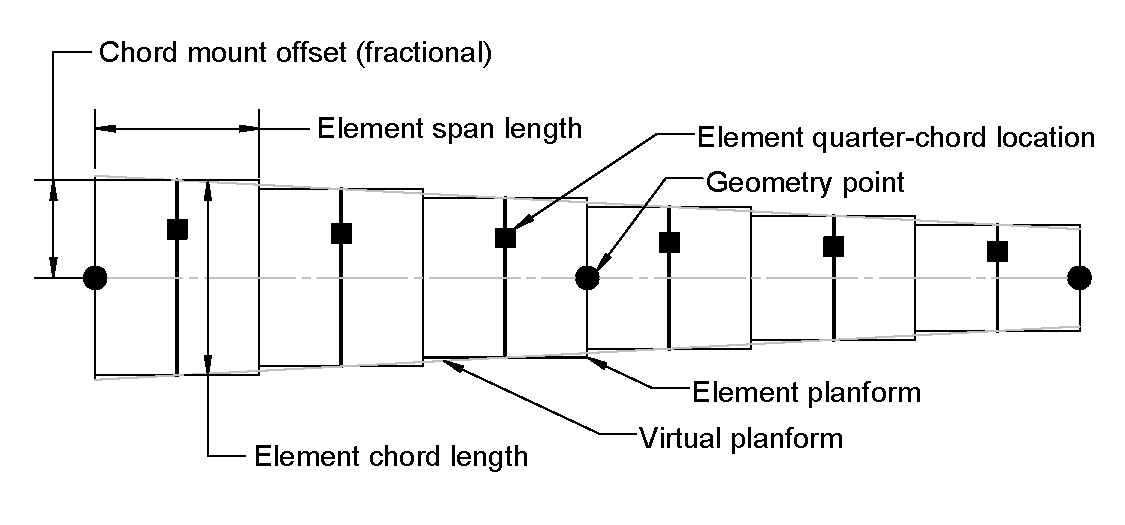
\includegraphics[width=0.7\textwidth]{thesis_alm-geometry}

    \caption{Actuator line geometry. Filled circles indicate points where
    geometry is defined whereas squares indicate actuator line element
    quarter-chord locations. Chord mount offset is defined as the distance from
    an element's leading edge to each geometry point in chord lengths, which was
    0.5 for both rotors modeled in this study.}

    \label{fig:AL-geom}
\end{figure}


\section{Determining inflow velocity}

In momentum methods, the inflow velocity is determined by solving for the axial
and angular induction factors \cite{Manwell2002}. However, using Navier--Stokes
methods, it is somewhat unclear how to calculate the velocity vector used to
compute the angle of attack and relative velocity, though we have access to much
more information about the flow. Sorensen and Shen used an actuator line
element's position to determine the inflow velocity for an axial-flow turbine
\cite{Sorensen2002}. Similarly, Shamsoddin and Porte-Agel use the velocity at a
blade element's location in their actuator line simulation of a vertical-axis
turbine using LES \cite{Shamsoddin2014}. NREL's SOWFA ALM for OpenFOAM also uses
the velocity at the actuator line element location for computing inflow velocity
and local angle of attack with no corrections \cite{Churchfield2013}.

Schito and Zasso developed an effective velocity model (EVM) for computing
actuator forces in Navier--Stokes simulations \cite{Schito2014}. Their EVM
proposes that inflow velocity should be sampled along a line perpendicular to
the mean relative flow direction. They ultimately determined that the sampling
line should be 1.5 chord lengths upstream of the actuator point (i.e.
quarter-chord location). A sampling line was chosen to be 5 times the local mesh
cell length. Finally, an angle of attack correction was proposed
\begin{equation}
    \Delta \alpha = \frac{c}{M} (1.2553 - 0.0552 C_d) C_l,
    \label{eq:EVM-dalpha}
\end{equation}
where $c$ is the chord length, $M$ is the mesh size, and $C_l$ and $C_d$ are the
lift and drag coefficients, respectively. Note that the constants in
Equation~\ref{eq:EVM-dalpha} were determined from a calibration with 2-D
blade-resolved CFD for a NACA 0012 foil and are not assumed to be universal.

The EVM, despite showing robustness for its chosen validation case,
unfortunately involves determination of two unknown tuning parameters. To avoid
the additional effort and uncertainty in determining these, the inflow velocity
was sampled at the element quarter-chord location using OpenFOAM's
\texttt{interpolationCellPoint} class, which provides a linear weighted
interpolation using cell values. This algorithm helps keep the sampled velocity
``smooth'' compared with using the cell values themselves, especially when
elements are moving in space as they are in a turbine, since meshes will likely
have a cell size on the same order as the chord length, and will move on the
order of one cell length per time step.


\section{Static foil coefficient data}

Static input foil coefficient data were taken from Sheldahl and
Klimas~\cite{Sheldahl1981}---a popular database developed for CFTs, which
contains values over a wide range of Reynolds numbers. The Sheldahl and Klimas
dataset has some limitations, namely that data for some foil and/or Reynolds
numbers were ``synthesized'' numerically from other measurements. Despite its
flaws, this dataset is the likely most comprehensive available with respect to
variety of profiles and ranges of Reynolds numbers. Surprisingly, considering
the maturity and popularity of NACA foils, data remains scarce, especially for
$Re_c \sim 10^5$.

NACA 0021 coefficients were used for both turbines, despite the fact that the
UNH-RVAT is constructed from NACA 0020 foils, as a NACA 0020 dataset is not
available---it is assumed the small difference in foil thickness is negligible.
Since pitching moment data were only available at limited Reynolds numbers, two
datasets were used: The lowest for $Re_c \leq 3.6 \times 10^5$ and highest $Re_c
\geq 6.8 \times 10^5$. For each actuator line element, blade chord Reynolds
number is computed based on the sampled inflow velocity, and the static
coefficients are then interpolated linearly within the database.


\section{Force projection}

After the force on the ALE from the flow is calculated, it is then projected
back onto the flow field as a source term in the momentum equation. To avoid
instability due to steep gradients, the source term is tapered from its maximum
value away from the element location by means of a spherical Gaussian function.
The width of this function $\eta$ is controlled by a single parameter
$\epsilon$, which is then multiplied by the actuator line element force and
imparted on a cell with distance $| \vec{r} |$ from the actuator line element
quarter chord location:
\begin{equation}
    \eta = \frac{1}{\epsilon^3 \pi^{3/2}} \exp
    \left[ - \left( \frac{| \vec{r} |}{\epsilon} \right)^2 \right].
    \label{eq:projection}
\end{equation}

Troldborg~\cite{Troldborg2008} proposed that the Gaussian width should be set to
twice the local cell length $\Delta x$ in order to maintain numerical stability.
Schito and Zasso \cite{Schito2014} found that a projection $\epsilon$ equal to
the local mesh length was optimal. Jha et al.~\cite{Jha2014} investigated the
ideal projection width for HAWT blades, recommending an equivalent elliptic
planform be constructed and used to calculate a spanwise $\epsilon$
distribution.

Martinez-Tossas and Meneveau \cite{Martinez-Tossas2015b} used a 2-D potential
flow analysis to determine that the optimal projection width for a lifting
surface is 14--25\% of the chord length. The width due to the wake caused by the
foil drag force was recommended to be on the order of the momentum thickness
$\theta$, which for a bluff body or foil at large angle of attack is related to
the drag coefficient ($O(1)$) by \cite{TennekesAndLumley}
\begin{equation}
    C_d = 2 \theta / l,
    \label{eq:mom-thickness}
\end{equation}
where $l$ is a reference length, e.g., diameter for a cylinder or chord length
for a foil.

Using these guidelines, three Gaussian width values were determined: one
relative to the chord length, one to the mesh size, and one to the momentum
thickness due to drag force. Each three were computed for all elements at each
time step, and the largest was chosen for the force projection algorithm. Using
this adaptive strategy, fine meshes could benefit from the increased accuracy of
more concentrated momentum sources, and coarse meshes would be protected from
numerical instability.

The Gaussian width due to mesh size $\epsilon_{\mathrm{mesh}}$ was determined
locally on an element-wise basis by estimating the size of the cell containing
the element as
\begin{equation}
    \Delta x \approx \sqrt[3]{V_\mathrm{cell}},
\end{equation}
where $V_\mathrm{cell}$ is the cell volume. To account for the possibility of
non-unity aspect ratio cells, an additional factor $C_\mathrm{mesh}$ was
introduced, giving
\begin{equation}
    \epsilon_{\mathrm{mesh}} = 2C_\mathrm{mesh} \Delta x.
\end{equation}
$C_{\mathrm{mesh}}$ was set to 2.0 for the simulations presented
here---determined by trial-and-error to provide stability on the finest grids.
However, in the ALM code $C_{\mathrm{mesh}}$ is selectable at run time for each
profile used.


\section{Unsteady effects}

In the context of a turbine---especially a cross-flow turbine---the actuator
lines will encounter unsteady conditions, both in their angle of attack and
relative velocity. These conditions necessitate the use of unsteady aerodynamic
models to augment the static foil characteristics, both to capture the time
resolved response of the attached flow loading and effects of flow acceleration,
also know as added mass. Furthermore, the angles of attack encountered by a CFT
blade will often be high enough to encounter dynamic stall (DS). It is therefore
necessary to model both unsteady attached and detached flow to obtain accurate
loading predictions.


\subsection{Dynamic stall}

Dynamic stall is encountered when the blade angle of attack changes rapidly in
time and exceeds a certain threshold, often near the static stall angle
\cite{McCroskey1981}. The stall is characterized by an initial increase in lift
beyond static values as a vortex is shed from the foil's leading edge, after
which a drop in lift and large nose-down pitching moment occurs as the vortex is
advected downstream. As the angle of attack drops below the critical value, flow
reattaches, closing the so-called hysteresis loop. Dynamic stall has been shown
to be a significant positive contributor to performance in CFTs \cite{Para2002,
    Urbina2013}, therefore an accurate model is key.

DS models were first developed to improve predictive capability for helicopter
rotors, on which DS has significant effects on maneuverability and operational
envelope \cite{Bousman2000}. A summary of dynamic stall models developed for
helicopter rotors is presented in \cite{Leishman2006}. The simplest dynamic
stall models rely on semi-empirical correlations, e.g., the Gormont model
\cite{Gormont1973}, developed at the Boeing--Vertol Company. Several variants of
the Gormont model were developed for vertical-axis wind turbines, with varying
degrees of success; a summary is presented in \cite{Para2002}.

Leishman and Beddoes (LB) \cite{Leishman1989} developed a semi-empirical model
for unsteady aerodynamics and dynamic stall, which is derived from the
phenomenology of the physics instead rather than pure empiricism. Beddoes then
updated the model to the so-called third generation or ``3G'' version
\cite{Beddoes1993}. The LB DS models can be summarized conceptually based on the
following principles:
\begin{itemize}
    \item Dynamic conditions cause a time lag in effective angle of attack and
    lift force.

    \item Separation is determined by the Kirchoff flow approximation, which is
    also used to parameterize the normal force coefficient table based on the
    trailing edge separation point. This separation point also encounters a time
    lag.

    \item The separation initiates a vortex shedding cycle that causes an
    overshoot and subsequent undershoot in lift before returning to an attached
    flow condition.
\end{itemize}

Sheng et al. \cite{Sheng2008} developed an LB DS model variant targeted at low
Mach numbers. This model, along with the original and 3G LB DS model variants,
was tested for its effectiveness in cross-flow turbine conditions by Dyachuk et
al.~\cite{Dyachuk2014}, who concluded that the Sheng et al. variant results
matched most closely with experiments. In a similar study, the Sheng et al.
model also faired better than the Gormont model \cite{Dyachuk2015}, which
inspired its adoption here for the ALM.

Before the dynamic stall subroutine is executed, the static profile data for
each element is interpolated linearly based on local chord Reynolds number. The
profile data characteristics---static stall angle, zero-lift drag coefficient,
and separation point curve fit parameters---are then recomputed each time step
such that the effects of Reynolds number on the static data are included.

Inside the ALM, angle of attack is sampled from the flow field rather than
calculated based on the geometric angle of attack. Therefore, the implementation
of the LB DS model was such that the equivalent angle of attack
$\alpha_\mathrm{equiv}$ was taken as the sampled rather than the lagged
geometric value. A similar implementation was used by Dyachuk et al.
\cite{Dyachuk2015a} inside a vortex model.


\subsection{Added mass}

A correction for added mass effects, or the effects due to accelerating the
fluid, was taken from Strickland et al.~\cite{Strickland1981}, which was
derived by considering a pitching flat plate in potential flow. In the blade
element coordinate system, the normal and chordwise (pointing from trailing to
leading edge, which is opposite the $x$-direction used by Strickland \emph{et
    al.}) coefficients due to added mass are
\begin{equation}
    C_{n_\mathrm{AM}} = -\frac{\pi c \dot{U_n}}{8 | U_\mathrm{rel} |^2},
\end{equation}
and
\begin{equation}
    C_{c_\mathrm{AM}} = \frac{\pi c \dot{\alpha} U_n }{8 | U_\mathrm{rel} |^2},
\end{equation}
respectively, where $U_n$ is the normal component of the relative velocity, and
dotted variables indicate time derivatives, which were calculated using a simple
first order backward finite difference. Similarly, the quarter-chord moment
coefficient due to added mass was calculated as
\begin{equation}
    C_{m_\mathrm{AM}} = -\frac{C_{n_\mathrm{AM}}}{4}
        - \frac{U_n U_c}{8 | U_\mathrm{rel} |^2},
\end{equation}
where $U_c$ is the chordwise component of relative velocity. Note that the
direction of positive moment is ``nose-up,'' which is opposite that used by
Strickland et al..

The normal and chordwise added mass coefficients translate to lift and drag
coefficients by
\begin{equation}
    C_{l_\mathrm{AM}} = C_{n_\mathrm{AM}} \cos \alpha + C_{c_\mathrm{AM}} \sin
    \alpha,
\end{equation}
and
\begin{equation}
    C_{d_\mathrm{AM}} = C_{n_\mathrm{AM}} \sin \alpha - C_{c_\mathrm{AM}} \cos
    \alpha,
\end{equation}
respectively. The added mass coefficients were then added to those calculated by
the dynamic stall model.


\section{Flow curvature corrections}

The rotating blades of a cross-flow turbine will have non-constant chordwise
angle of attack distributions due to their circular paths---producing so-called
flow curvature effects~\cite{Migliore1980}. This makes it difficult to define a
single angle of attack for use in the static coefficient lookup tables.
Furthermore, this effect is more pronounced for high solidity ($c/R$) turbines.
Two different flow curvature corrections were considered: one derived in Goude
\cite{Goude2012} and one by Mandal and Burton \cite{Mandal1994}.

The Goude correction is derived by considering a flat plat moving along a
circular path in potential flow, for which the effective angle of attack
including flow curvature effects is given by
\begin{equation}
    \alpha = \delta + \arctan \frac{V_\mathrm{abs} \cos(\theta_b -
        \beta)}{V_\mathrm{abs} \sin(\theta_b - \beta) + \Omega R} - \frac{\Omega
        x_{0r}c}{V_\mathrm{ref}} - \frac{\Omega c}{4 V_\mathrm{ref}},
    \label{eq:Goude-curvature}
\end{equation}
where $\delta$ is the blade pitch angle, $V_\mathrm{abs}$ is the magnitude of
the local inflow velocity at the blade, $\theta_b$ is the blade azimuthal
position, $\beta$ is the direction of the inflow velocity, $\Omega$ is the
turbine's angular velocity, $R$ is the blade element radius, $x_{0r}$ is a
normalized blade attachment point along the chord (or fractional chord distance
of the mounting point from the quarter-chord), $c$ is the blade chord length,
and $V_\mathrm{ref}$ is the reference flow velocity for calculating angle of
attack.

In the actuator line model, each element's angle of attack is calculated using
vector operations, which means the first two terms in
Equation~\ref{eq:Goude-curvature} are taken care of automatically since each
element's inflow velocity, chord direction, and element velocity vectors are
tracked. Therefore, the last two terms in Equation~\ref{eq:Goude-curvature} were
simply added to the scalar angle of attack value. Note that for a cross-flow
turbine, this correction effectively offsets the angle of attack, which
therefore increases its magnitude on the upstream half of the blade path, and
decreases its magnitude on the downstream half, where the angle of attack is
negative.

The Mandal--Burton flow curvature correction assumes that since the blade is
encountering a curvilinear flow, it can be treated as having virtual camber.
They introduce a factor to describe the variation of angle of attack from the
leading to trailing edge
\begin{equation}
    \Delta \alpha = \alpha_\mathrm{TE} - \alpha_\mathrm{LE},
    \label{eq:Mandal-Burton-alpha-diff}
\end{equation}
where TE and LE subscripts denote the values of angle of attack at the trailing
and leading edge, respectively. Calculating these values for an actuator line
element can be done by tracking the leading and trailing edge locations and
velocities, then performing the same vector arithmetic used to calculate the
quarter-chord angle of attack.

An incidence correction factor
\begin{equation}
    \alpha_c = \arctan \left( \frac{1 - \cos (\Delta \alpha / 2)}{\sin (\Delta
        \alpha / 2)} \right)
    \label{eq:Mandal-Burton-alpha-corr}
\end{equation}
is introduced and added to the uncorrected angle of attack. Like the Goude
model, $\alpha_c$ is positive on the upstream half of the turbine rotation and
negative on the downstream half.

It was determined that the Goude model performed best with respect to matching
the near-wake characteristics measured in the experiments, while the performance
predictions from both flow curvature models were relatively close to each other.
Thus, the Goude model was used for all simulations reported here.


\section{End effects}

Helmholtz's second vortex theorem states that vortex lines may not end in a
fluid, but must either form closed loops or extend to boundaries. Consequently
the lift distribution due to the bound vortex from foils of finite span must
drop to zero at the tips.

Glauert~\cite{Glauert1935} used Prandtl's lifting line theory \cite{Prandtl1927}
to develop a tip loss correction factor $F$ to be applied to the local lift of
an axial-flow rotor blade element:
\begin{equation}
    F = \frac{2}{\pi} \cos^{-1} \left[ \exp \left( - \frac{N (R-r)}{2R \sin
        \phi_R} \right) \right],
\end{equation}
where $F$ is the correction factor applied to the local lift, $N$ is number of
blades, $R$ is the rotor radius, $r$ is the local blade element radius, and
$\phi_R$ is the flow angle at the tip.

The Glauert correction was further refined for horizontal-axis wind turbines by
Shen et al. \cite{Shen2005a} as
\begin{equation}
    F_1 = \frac{2}{\pi} \cos^{-1} \left[ \exp \left( -g \frac{N (R-r)}{2R \sin
    \phi_R} \right) \right],
\end{equation}
where $g$ is an additional function depending on the tip speed ratio and two
tuning constants:
\begin{equation}
    g = \exp [ -c_1 (B \lambda - c_2) ].
\end{equation}

Despite their success for the blade element analysis of axial-flow rotors, these
corrections both depend on rotor parameters---tip speed ratio, number of blades,
element radius, tip flow angle---that do no necessarily translate directly to
the geometry and flow environment of a cross-flow rotor. Therefore, a more
general end effects model was sought.

From Prandtl's lifting line theory, the geometric angle of attack $\alpha$ of a
foil with an arbitrary circulation distribution can be expressed as a function
of nondimensional span $\theta$ as \cite{Anderson2001}
\begin{equation}
    \alpha (\theta) = \frac{2S}{\pi c (\theta)}
    \sum_1^N A_n \sin \theta
    + \sum_1^N n A_n \frac{\sin n \theta}{\sin \theta}
    + \alpha_{L = 0}(\theta),
    \label{eq:lifting-line}
\end{equation}
where $S$ is the span length, $c(\theta)$ is the chord length, and $N$ is the
number of locations or elements sampled along the foil. This relationship can be
rearranged into a matrix equation to solve for the unknown Fourier coefficients
$A_n$,
\begin{equation}
    [\alpha_m ] - \alpha_{L=0} = [D_{mn}][A_n],
\end{equation}
where
\begin{equation}
    D_{mn} = \sum_1^N \left[ \frac{2b}{\pi c_m} \sin n \theta_m + n \frac{\sin n
        \theta_m}{\sin \theta_m} \right].
\end{equation}

With the Fourier coefficients, the circulation distribution can be calculated as
\begin{equation}
    \Gamma (\theta) = 2SU_\infty \sum_1^N A_n \sin n \theta,
\end{equation}
which, via the Kutta--Joukowski theorem, provides the lift coefficient
distribution
\begin{equation}
    C_l(\theta) = \frac{-\Gamma (\theta)}{\frac{1}{2} c U_\infty}.
\end{equation}

We can therefore compute a correction function based on the normalized spanwise
lift coefficient distribution
\begin{equation}
    F = C_l(\theta)/C_l(\theta)_{\max},
\end{equation}
which will be in the range $[0, 1]$, similar to the Glauert corrections, but
does not contain rotor parameters.

The correction functions for the standard Glauert and lifting line methods are
plotted for comparison in Figure~\ref{fig:end-effects}. Function values were
computed using the UNH-RVAT geometry, $\lambda = \lambda_0 = 1.9$, and a 20
degree tip angle of attack. Both end effects corrections produce similar results
for this specific case, which gives confidence that the lifting line method will
produce reasonable results without the uncertainty of translating axial-flow to
cross-flow rotor parameters.

\begin{figure}
    \centering

    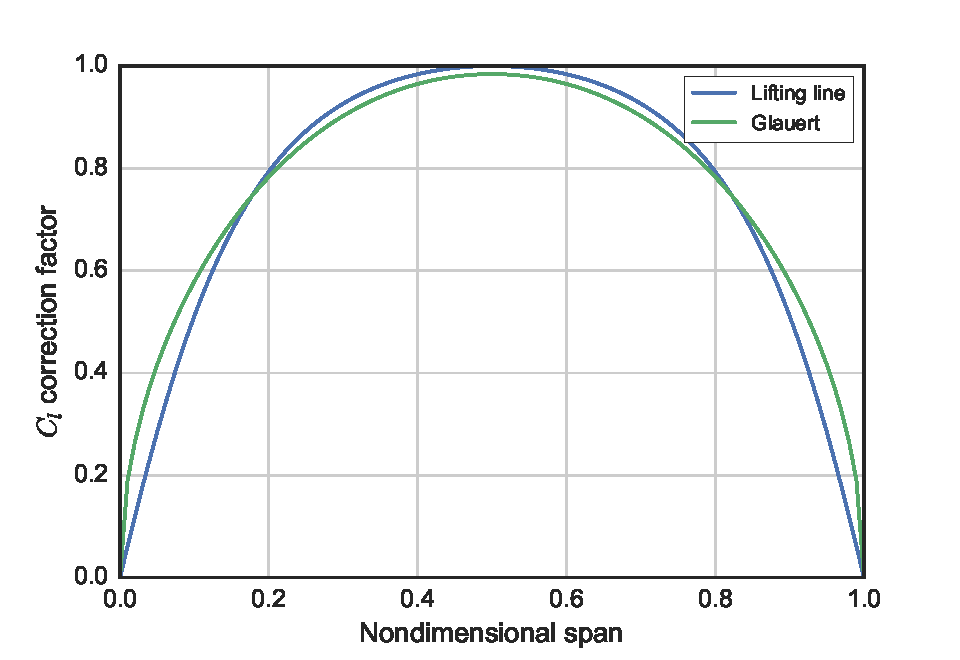
\includegraphics[width=0.65\textwidth]{end-effects_rvat-20-deg}

    \caption{End effect correction function values for the Glauert and lifting
        line methods using UNH-RVAT parameters at 20 degrees tip angle of attack and
        $\lambda=1.9$.}

    \label{fig:end-effects}
\end{figure}


\section{Software implementation}

The US National Renewable Energy Laboratory (NREL) has developed and released an
actuator line modeling library, SOWFA~\cite{Churchfield2014b}, for simulating
horizontal-axis wind turbine arrays using the OpenFOAM finite volume CFD
library. OpenFOAM is free, open-source, widely used throughout industry and
academia, and has grown a very active support community around itself
\cite{Bachant2015-CFD-online}. Though SOWFA is also open-source, and has the
ability to be coupled to NREL's FAST HAWT BEM code, its mostly procedural style
would have required significant effort and duplicate code to adapt for
cross-flow turbines. Thus, a new and more general ALM library was developed from
the ground up that could model both cross- and axial-flow turbines, as well as
standalone actuator lines. The actuator line model developed here, dubbed
turbinesFoam \cite{Bachant2016-turbinesFoam-v0.0.7}, was also written as an
extension library for OpenFOAM, and was developed freely and openly from its
inception in order to increase community engagement and research efficiency.

turbinesFoam was written in OpenFOAM's style, using OpenFOAM's
\texttt{fvOptions} framework for adding source terms to equations at
runtime---see Listing~\ref{lst:fvOptions} for an example implementation within
the Navier--Stokes' momentum equation. Using the \texttt{fvOptions} framework
allows the CFT-ALM to be added to many of the solvers included in OpenFOAM,
meaning it can be readily used with RANS or LES, multiphase models (e.g., for
simulating the free surface in MHK installations), and even with heat transfer.
This is in contrast to SOWFA's implementation, which requires custom flow
solvers to be developed and maintained.

\begin{lstlisting}[float,language=C++,caption=Adding source terms to the momentum equation in OpenFOAM.,label=lst:fvOptions]
    tmp<fvVectorMatrix> UEqn
    (
        fvm::ddt(U)
        + fvm::div(phi, U)
        + turbulence->divDevReff(U)
        ==
        fvOptions(U)
    );
\end{lstlisting}

OpenFOAM and turbinesFoam are written in the C++ programming language, which
follows the object oriented programming paradigm. This characteristic helped
modularize the ALM code for increased readability and reuse. In turbinesFoam, a
turbine is a software object that is composed of actuator line objects, which
themselves are composed of actuator line element objects. Structuring the code
this way allows isolation and reuse of the functionality of individual
components. For example, the actuator line object was written such that is could
be used outside the turbine context to ensure it produces the correct forcing,
without adding the complexity of rotation, other actuator lines, etc. that would
be present in a turbine rotor. The very same actuator line objects can be used
in both axial-flow and cross-flow rotors, without having to copy code from one
to the other. In contrast, the actuator line model in SOWFA uses a single
software object to represent an entire array of turbines, which necessitates
iterating through many nested lists down to the element level, which can be
confusing to read.

OpenFOAM's data structures are designed to be inherently parallel via message
passing interface (MPI). By working within the library infrastructure the ALM
code was easily parallelized, which will facilitate its deployment on high
performance computing clusters for large flow simulations.

Since all applications are run from a command line and all input data is text
based, automation and integration with other tools is relatively
straightforward. Future enhancements could include coupling with software for
generating static foil data, e.g., XFOIL~\cite{Drela1989} or other OpenFOAM
solvers, turbine controller models, structural analysis codes, and optimization
tools, e.g., SNL's DAKOTA \cite{AdamsBaumanBohnhoffEtAl2009} or
OpenMDAO~\cite{Gray2010}, for both individual turbines and array layouts.


\section{Results}

Both the high solidity UNH-RVAT and medium-low solidity RM2 turbines were
modeled using the ALM inside a Reynolds-averaged Navier--Stokes (RANS)
simulation, closed with the standard $k$--$\epsilon$ turbulence model. These
rotors provide diverse parameters, which helped evaluate the robustness of the
ALM. The simulations were performed inside a domain similar in size to that used
in \cite{Bachant2016-BR-CFD} to mimic the tow tank experiments (3.66 m wide,
2.44 m tall, 1.52 m upstream and 2.16 m downstream), with similar velocity
boundary conditions: 1 m/s inflow, no-slip (fixed to 1 m/s) walls and bottom,
and a rigid slip condition for the top, to approximate some effects of the tow
tank's free surface. Simulations were run for a total of 6 seconds, with the
latter half used to calculate performance and wake statistics.
Pressure--velocity coupling for the momentum equation was achieved using the
PISO (pressure implicit splitting of operators) method. A slice of the mesh in
the $x$--$y$ plane is shown in Figure~\ref{fig:ALM-mesh}.

\begin{figure}
    \centering

    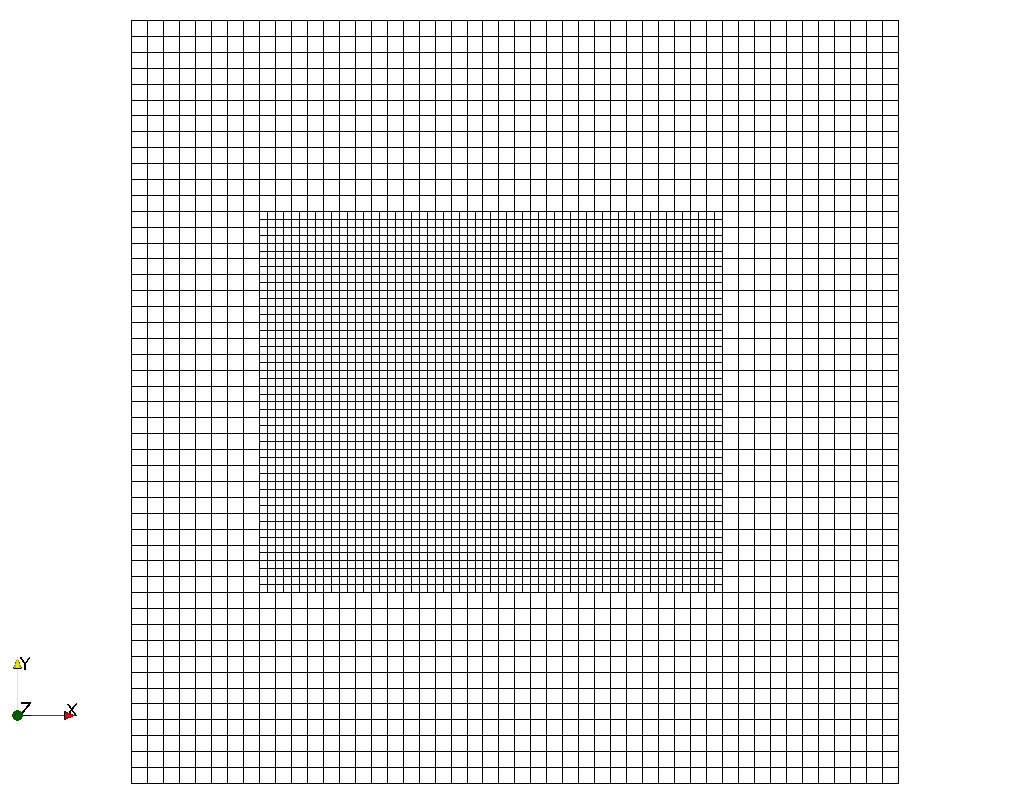
\includegraphics[width=0.8\textwidth]{thesis_alm-mesh}

    \caption{$x$--$y$ planar slice of the mesh used for the ALM RANS
        simulations.}

    \label{fig:ALM-mesh}
\end{figure}

Similar numerical settings were used for each turbine as well. The Sheng et al.
DS model was used with the default coefficients given in \cite{Sheng2008}, and
the Goude flow curvature correction was employed. A second order backward
difference was used for advancing the simulation in time, and second order
linear schemes were used for the majority of the terms' spatial discretizations.
The only major difference between the two simulation configurations was that the
end effects model was deactivated for the RM2, since it reduced $C_P$ far below
the experimental measurements. This modification is consistent with the RM2
blades' higher aspect ratio (15 versus the UNH-RVAT's 7.1) and tapered planform,
though will need to be investigated further. The number of elements per actuator
line was set to be approximately equal to the total span divided by the Gaussian
force projection width $\epsilon$. Case files for running all the simulations
presented here with OpenFOAM 3.0.x are available from
\cite{Bachant2016-UNH-RVAT-turbinesFoam-v1.0.0,
Bachant2016-RM2-turbinesFoam-v1.0.0,
Bachant2016-UNH-RVAT-turbinesFoam-v1.0.0-LES}.

The same foil coefficient data were used for all simulations---those for a NACA
0021 as reported by Sheldahl and Klimas \cite{Sheldahl1981}. Each rotor's shaft
was assumed to have a drag coefficient $C_d = 1.1$, and the blade support strut
end element drag coefficients were set to 0.05, to approximate the effects of
separation in the corners of the blade--strut connections.

Since the ALM is intended to be an engineering tool when coupled with RANS, it
was assumed that information about tip speed ratio due to control details---that
is, sinusoidally oscillating $\lambda$---would not be known a priori, and was
excluded, unlike the 3-D blade-resolved cases reported in
\cite{Bachant2016-BR-CFD}. Note that a systematic investigation of the effects
of sinusoidal $\lambda$ was not undertaken, but for the UNH-RVAT a one to two
percentage point increase in $C_P$ was observed when running with similar
parameters as the blade-resolved simulation.

Compared to 3-D blade-resolved RANS, the ALM can solve a standalone turbine case
on the order of 0.1 CPU hours per second of simulated time versus 1,000 CPU
hours per second---a savings of 4 orders of magnitude.


\subsection{Verification}

Verification for sensitivity to spatial and temporal grid resolution was
performed for both the UNH-RVAT and RM2 RANS cases at their optimal tip speed
rations, the results from which are plotted in
Figure~\ref{fig:RVAT-ALM-verification} and
Figure~\ref{fig:RM2-ALM-verification}, respectively. Similar to the verification
strategy employed in \cite{Bachant2016-BR-CFD}, the mesh topology was kept
constant, and the resolution was scaled proportional to the number of cells in
the $x$-direction $N_x$ for the base hexahedral mesh. Both models displayed low
sensitivity to the number of time steps per revolution. Spatial grid dependence,
however, was more important.

Final spatial grid resolutions were chosen as $N_x=48$ for both the UNH-RVAT and
RM2 cases. Time steps were chosen as $\Delta t = 0.01$ and $\Delta t = 0.005$
seconds for the UNH-RVAT and RM2 respectively, which correspond to approximately
200 steps per revolution. The chosen values should provide $C_P$ predictions
within one percentage point of the true solution, which is on the order of the
expanded uncertainty of the experimental measurements. Note that for computing
performance curves, the number of steps per revolution was kept constant, i.e.,
the time step was adjusted to $\Delta t = \Delta t_0 \lambda_0 / \lambda$.

\begin{figure}
    \centering

    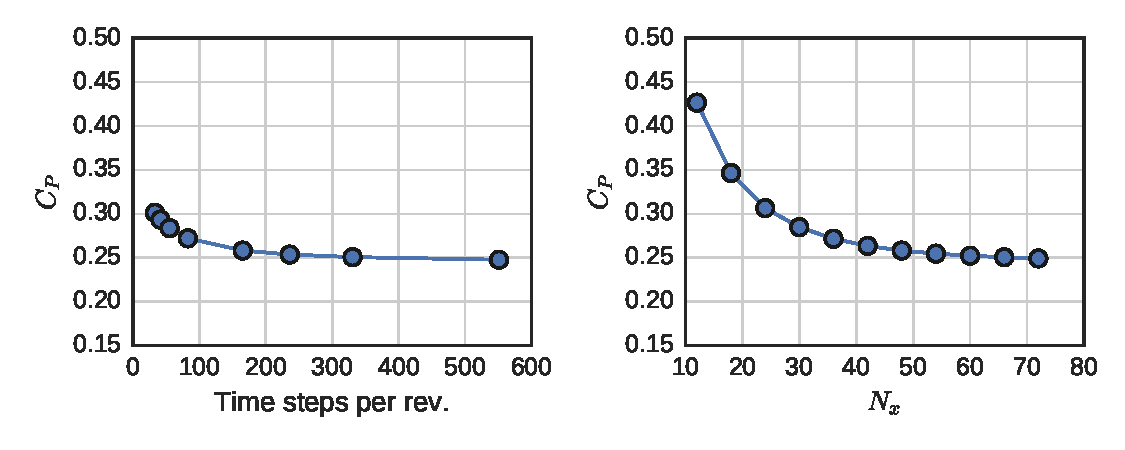
\includegraphics[width=0.7\textwidth]{RVAT-ALM_verification}

    \caption{Temporal (left) and spatial (right) grid resolution sensitivity
        results for the UNH-RVAT ALM RANS model.}

    \label{fig:RVAT-ALM-verification}
\end{figure}

\begin{figure}
    \centering

    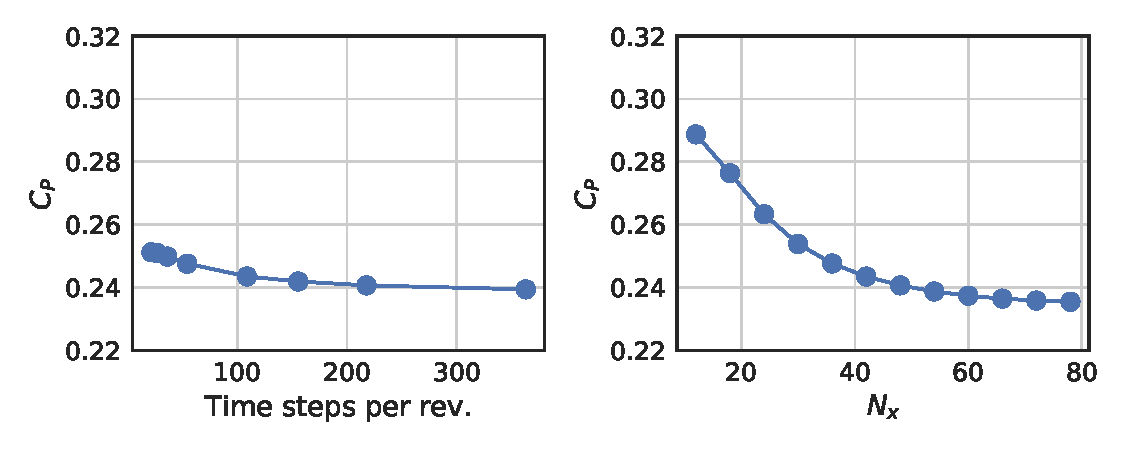
\includegraphics[width=0.7\textwidth]{RM2-ALM_verification}

    \caption{Temporal (left) and spatial (right) grid resolution sensitivity
        results for the RM2 ALM RANS model.}

    \label{fig:RM2-ALM-verification}
\end{figure}


\subsection{UNH-RVAT RANS}

Power and drag coefficient curves are plotted for the UNH-RVAT in
Figure~\ref{fig:RVAT-ALM-perf-curves}. The ALM was successful at predicting the
performance tip speed ratios up to $\lambda_0$, which suggests that dynamic
stall was being modeled accurately, but $C_P$ was overpredicted at high
$\lambda$. This may have been caused by the omission of additional parasitic
drag sources such as roughness from exposed bolt heads located far enough from
the axis to have a large effect at high rotation rates, or an underestimation of
the blade--strut connection corner drag coefficient. In
\cite{Rawlings2008,Bachant2016-RM2-paper} it was shown how these losses can be
significant even with carefully smoothed struts and strut-blade connections.
Overprediction of performance at high tip speed ratio could also be a
consequence of the Leishman--Beddoes dynamic stall model, which can also be seen
in the Darrieus VAWT momentum model results shown in Figure 6.70 of
\cite{Para2002}.

\begin{figure}
    \centering

    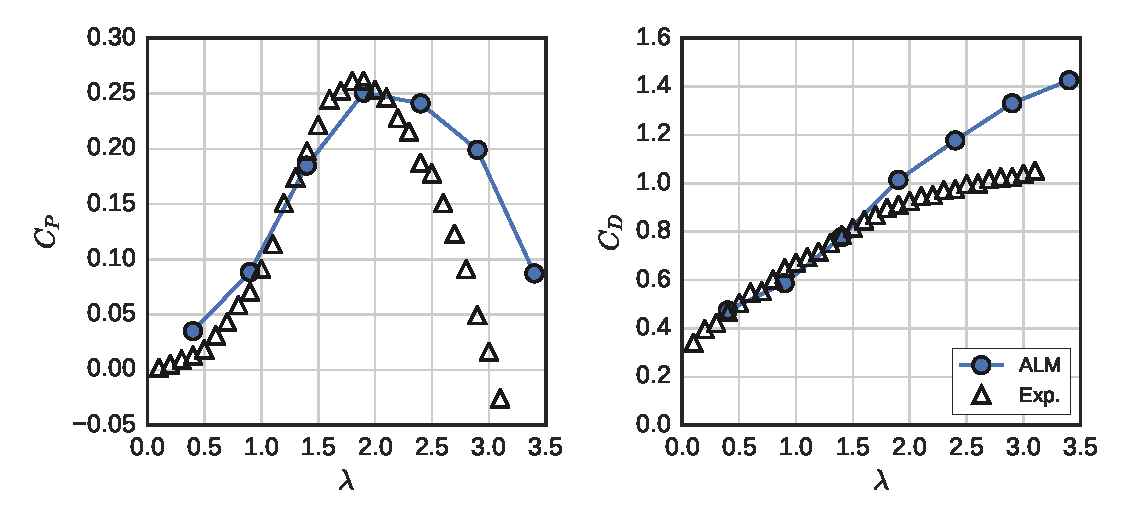
\includegraphics[width=0.7\textwidth]{RVAT-ALM_perf-curves}

    \caption{Power and drag coefficient curves computed for the UNH-RVAT using
        the actuator line model with RANS.}

    \label{fig:RVAT-ALM-perf-curves}
\end{figure}

Figure~\ref{fig:RVAT-ALM-meancontquiv} shows mean velocity field for the
UNH-RVAT computed by the ALM RANS model. The asymmetry was captured well, along
with some of the vertical flow due to blade tip vortex shedding, though the flow
structure is missing the detail present in the experiments and blade-resolved
RANS simulations. Overall, the wake appears to be over-diffused, which could be
a consequence of the relatively coarse mesh. Note that with the DS and flow
curvature corrections turned off, the direction of the mean swirling motion
reverses, which highlights the importance of resolving the correct azimuthal
location of blade loading.

\begin{figure}
    \centering

    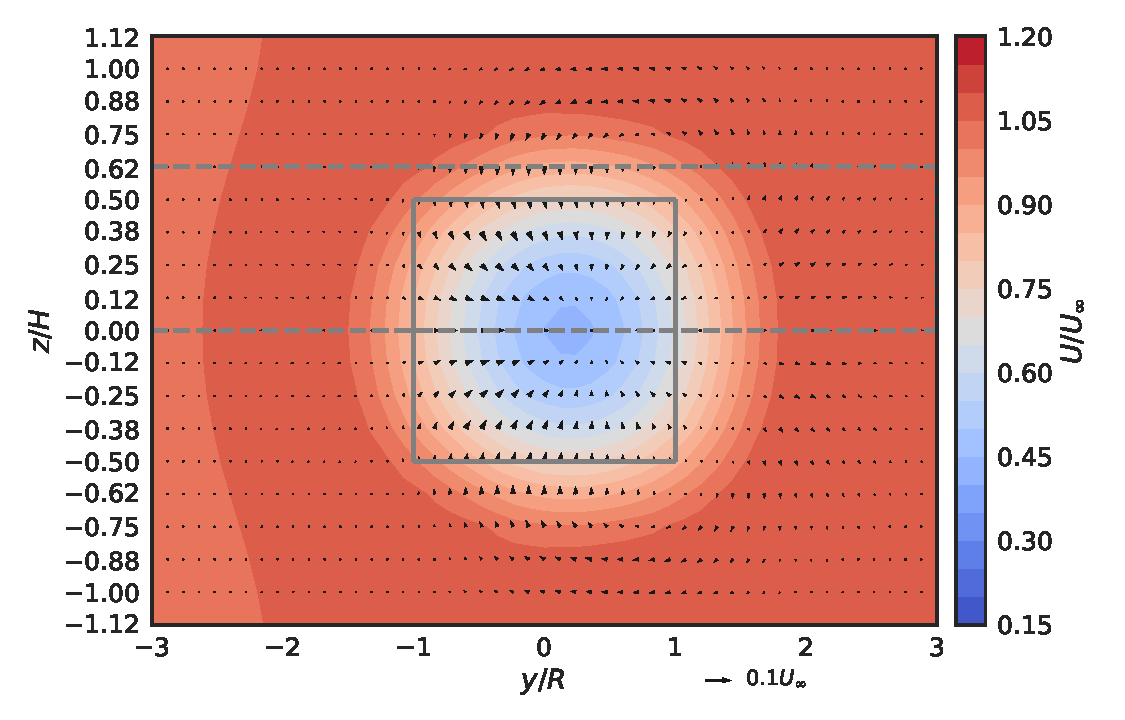
\includegraphics[width=0.75\textwidth]{RVAT-ALM_meancontquiv}

    \caption{UNH-RVAT mean velocity field at $x/D=1$ computed with the ALM
        coupled with a $k$--$\epsilon$ RANS model.}

    \label{fig:RVAT-ALM-meancontquiv}
\end{figure}

Turbulence kinetic energy contours (including resolved and modeled energy) are
shown in Figure~\ref{fig:RVAT-ALM-kcont}. The ALM was able to resolve the
concentrated area of $k$ on the $+y$ side of the turbine, but the turbulence
generated by the dynamic stall vortex shedding process is absent. This makes
sense since in the ALM, the DS model only modulates the body force term in the
momentum equation, which does not provide a mechanism for mimicking shed
vortices or turbulence.

\begin{figure}
    \centering

    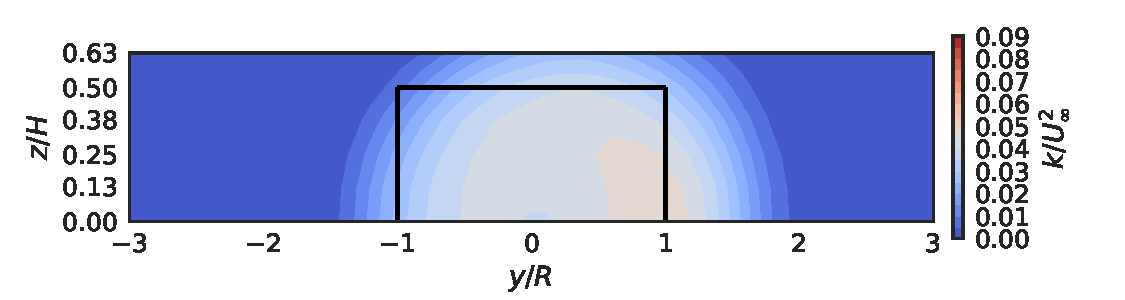
\includegraphics[width=0.7\textwidth]{RVAT-ALM_kcont}

    \caption{UNH-RVAT turbulence kinetic energy contours at $x/D=1$ predicted by
        the ALM inside a $k$--$\epsilon$ RANS model.}

    \label{fig:RVAT-ALM-kcont}
\end{figure}

Profiles of mean streamwise velocity and turbulence kinetic energy are shown in
Figure~\ref{fig:RVAT-ALM-profiles}. Here the over-diffused or over-recovered
characteristic of the mean velocity deficit seen in
Figure~\ref{fig:RVAT-ALM-meancontquiv} is more apparent. This effect is also
seen in the profile of $k$, where energy is smeared over the center region of
the rotor.

\begin{figure}
    \centering

    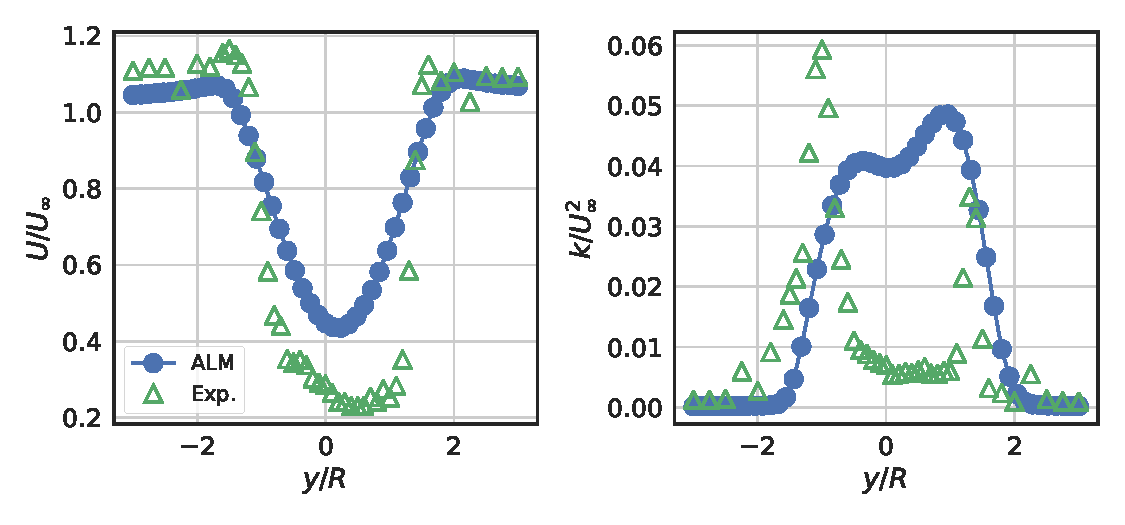
\includegraphics[width=0.7\textwidth]{RVAT-ALM_wake-profiles}

    \caption{Mean streamwise velocity (left) and turbulence kinetic energy
        (right) profiles at $z/H=0$ for the UNH-RVAT ALM.}

    \label{fig:RVAT-ALM-profiles}
\end{figure}

Weighted averages for the terms in the streamwise momentum equation were
computed identically as they were in \cite{Bachant2015-JoT,Bachant2016-BR-CFD},
and are plotted in Figure~\ref{fig:RVAT-ALM-recovery} along with the actuator
disk (AD) results from \cite{Bachant2015-JoT}, 3-D blade-resolved RANS results
from \cite{Bachant2016-BR-CFD} and experiments. The most glaring discrepancy is
the ALM's prediction of positive cross-stream advection, which is caused by the
lack of detail in the tip vortex shedding. The total for vertical advection,
however, is close to that predicted by the 3-D blade-resolved Spalart--Allmaras
model. Levels of turbulent transport due to eddy viscosity and deceleration due
to the adverse pressure gradient are between those predicted by the 3-D
blade-resolved $k$--$\omega$ SST and SA models. Overall, however, one might
expect the total wake recovery rate to be comparable between all models except
the actuator disk, which induces negative vertical advection, very little
turbulent transport, and has a positive pressure gradient contribution. These
results suggests the ALM would be an effective tool---much better than an
actuator disk---for assessing downstream spacing of subsequent CFTs, though
blade--vortex interaction for very tightly spaced rotors may not be captured, at
least on relatively coarse meshes as used here.

\begin{figure}
    \centering

    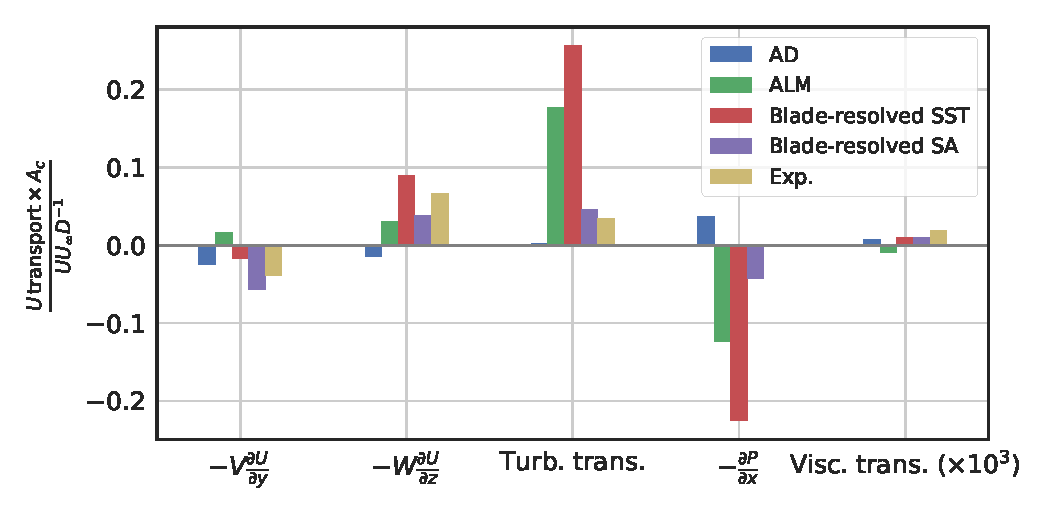
\includegraphics[width=0.7\textwidth]{RVAT-ALM_recovery-bar-chart}

    \caption{Weighted average momentum recovery terms for the actuator disk (AD)
        simulation from \cite{Bachant2015-JoT}, UNH-RVAT actuator line model with a
        $k$--$\epsilon$ RANS closure, the two 3-D blade resolved RANS models
        described in \cite{Bachant2016-BR-CFD}, and the experiments reported in
        \cite{Bachant2015-JoT}.}

    \label{fig:RVAT-ALM-recovery}
\end{figure}


\subsection{RM2 RANS}

Figure~\ref{fig:RM2-ALM-perf-curves} shows the performance curves computed for
the RM2 by the ALM, and those from the tow tank experiments. As with the high
solidity RVAT, $C_P$ is overpredicted at high $\lambda$. However, $\lambda_0$,
the tip speed ratio of peak power coefficient, is also shifted to the right.
This is indicative of inaccurate dynamic stall modeling, which could possibly be
attributed to one of the models' tuning constants, e.g., the time constant for
the lagged angle of attack. Limited ad hoc testing revealed that $C_P$ at
$\lambda_0$ was more accurately predicted with a lagged angle of attack time
constant roughly double the default value. This could be investigated further by
looking at the phase of, e.g., maximum $C_P$ peaks compared to the experimental
values (or possibly those from blade-resolved CFD), but for the present study
only mean values were considered.

\begin{figure}
    \centering

    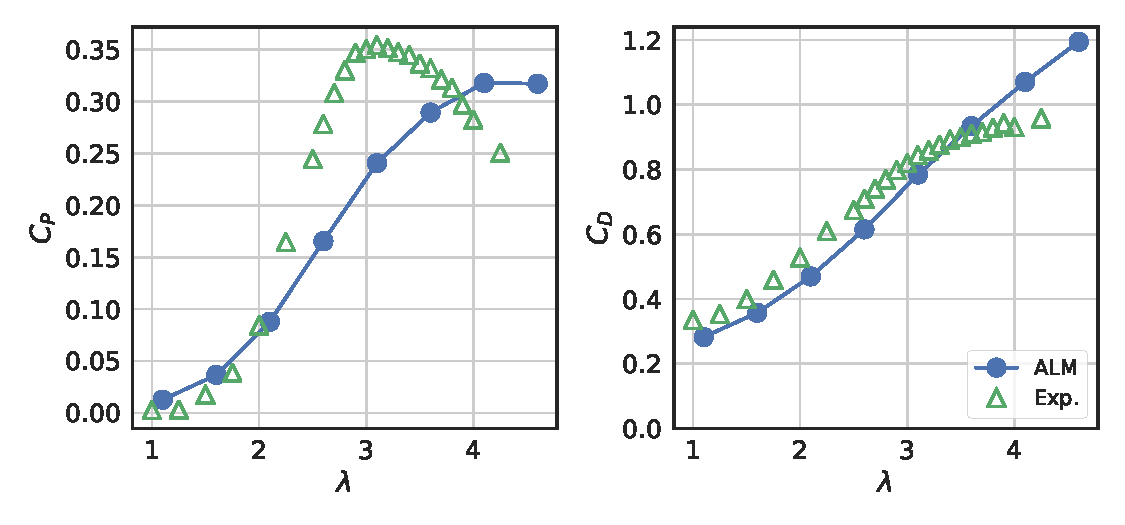
\includegraphics[width=0.7\textwidth]{RM2-ALM_perf-curves}

    \caption{Power and drag coefficient curves computed for the RM2 using the
        ALM.}

    \label{fig:RM2-ALM-perf-curves}
\end{figure}

Figure~\ref{fig:RM2-ALM-meancontquiv} shows the mean velocity field at 1 m
downstream or $x/D=0.93$ computed by the ALM for the RM2. The mean near-wake
structure looks similar to the RVAT ALM RANS case, but for the RM2, the lack of
detail from blade tip vortex shedding matches more closely with experiments.
However, the vertical flow towards the $x$--$y$ center plane was captured, which
is an important qualitative feature of both CFT near-wakes.

\begin{figure}
    \centering

    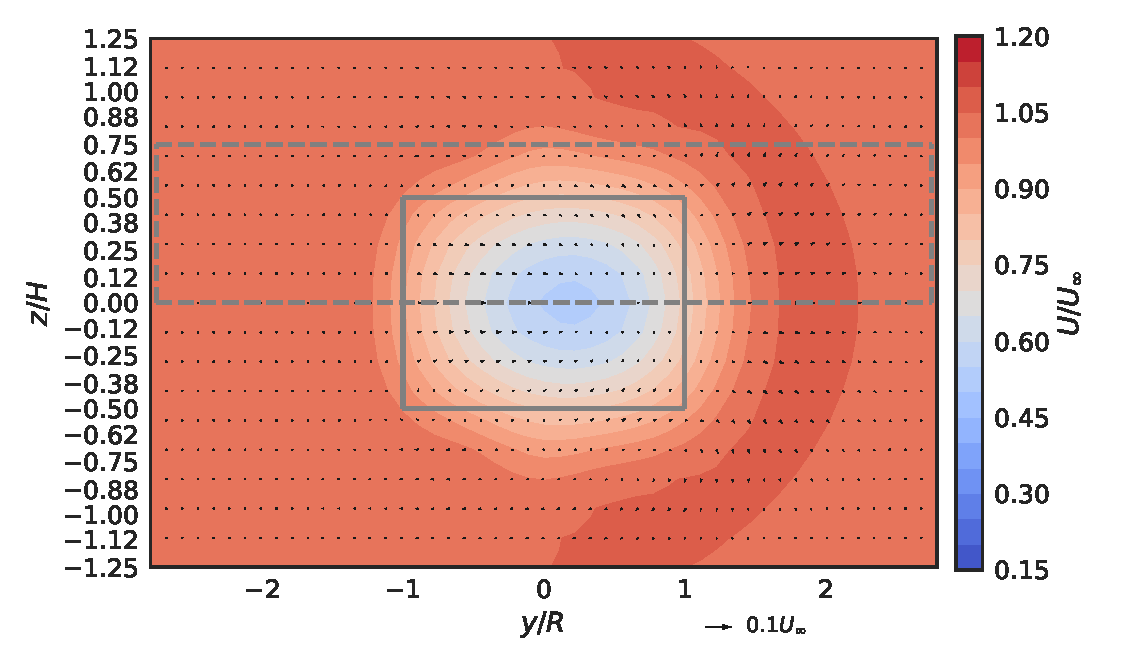
\includegraphics[width=0.75\textwidth]{RM2-ALM_meancontquiv}

    \caption{Mean velocity field at $x/D=0.93$ for the RM2 predicted by the
        ALM.}

    \label{fig:RM2-ALM-meancontquiv}
\end{figure}

Figure~\ref{fig:RM2-ALM-kcont} shows the ALM's turbulence kinetic energy
predictions in the near-wake of the RM2. Like for the UNH-RVAT, $k$ appears to
be concentrated on the $+y$ side of the rotor. However, overall levels of
turbulence are lower than for the UNH-RVAT, which is consistent with the
experimental results. However, turbulence generated by the RM2's blade tip
vortex shedding was not captured by the ALM.

\begin{figure}
    \centering

    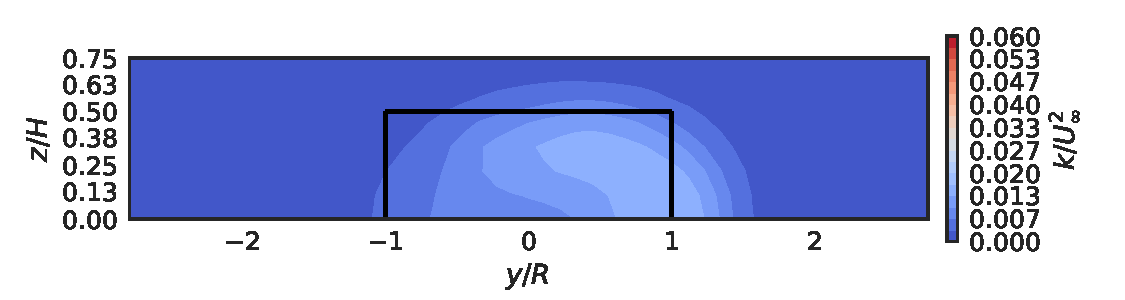
\includegraphics[width=0.7\textwidth]{RM2-ALM_kcont}

    \caption{Turbulence kinetic energy contours at $x/D=0.93$ behind the RM2
        predicted by the ALM.}

    \label{fig:RM2-ALM-kcont}
\end{figure}

Wake profiles at turbine mid-height in the $x$--$y$ center plane are shown in
Figure~\ref{fig:RM2-ALM-profiles}. Like the UNH-RVAT case, the mean velocity
deficit appears to be recovering too quickly, which may similarly be due to
coarseness of the grid or overprediction of the eddy viscosity. The peak in
turbulence kinetic energy on the $-y$ side of the turbine was also
underpredicted, though was much lower in magnitude compared to the UNH-RVAT,
even in the experimental measurements.

\begin{figure}
    \centering

    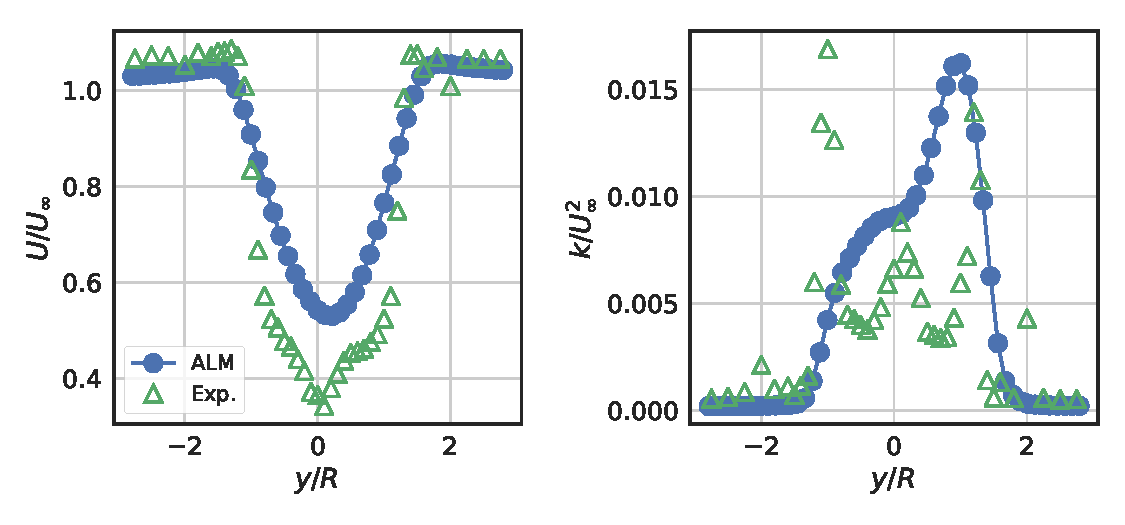
\includegraphics[width=0.7\textwidth]{RM2-ALM_wake-profiles}

    \caption{Mean streamwise velocity (left) and turbulence kinetic energy
    (right) profiles at $x/D=0.93$ and $z/H=0$ computed for the RM2 using the
    ALM inside a $k$--$\epsilon$ RANS model.}

    \label{fig:RM2-ALM-profiles}
\end{figure}

Finally, a similar mean streamwise momentum transport analysis was undertaken by
computing weighted sums of each term across the entire domain in the $y$--$z$
directions. Similar results as for the UNH-RVAT were obtained, i.e.,
cross-stream advection was predicted to be positive where it should have been
negative, vertical advection was predicted reasonably well, and turbulent
transport due to the eddy viscosity was also relatively large.

\begin{figure}
    \centering

    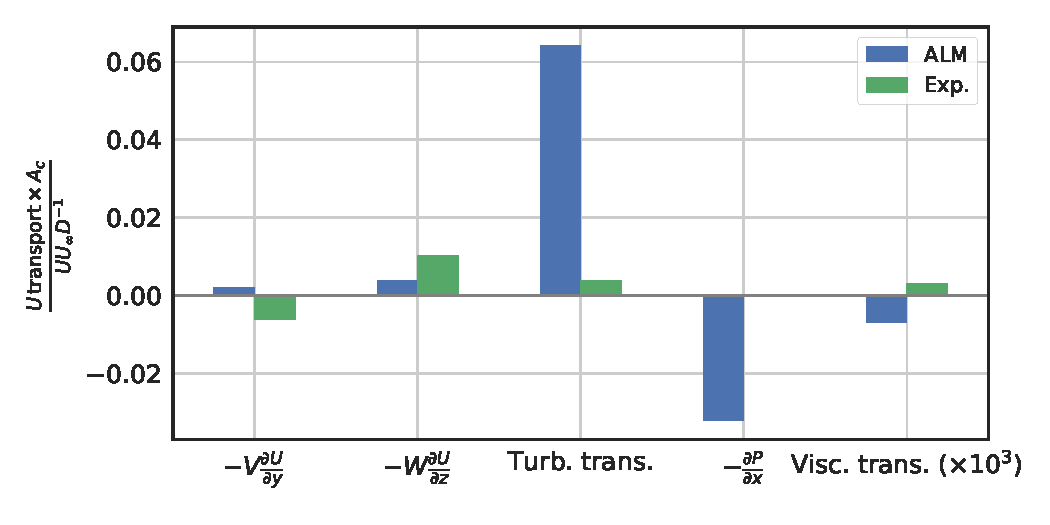
\includegraphics[width=0.7\textwidth]{RM2-ALM_recovery-bar-chart}

    \caption{Weighted average momentum recovery terms at $x/D=0.93$ for the RM2
        actuator line model with a $k$--$\epsilon$ RANS closure and the experiments
        described in \cite{Bachant2016-RM2-paper}.}

    \label{fig:RM2-ALM-recovery}
\end{figure}


\subsection{UNH-RVAT LES}

The state-of-the-art in high fidelity turbine array modeling uses the actuator
line method coupled with large eddy simulation (LES), which allows more of the
turbulent energy spectrum to be directly resolved, only requiring the dynamics
of the smallest scales---where dissipation occurs---to be computed by the
so-called subgrid-scale (SGS) model. Since the ALM LES approach has only been
reported in the literature for a very low Reynolds number 2-D CFT
\cite{Shamsoddin2014}, and CFTs may provide unique opportunities to array
optimization, which could be explored with LES, it was of interest to determine
how well the ALM coupled with LES might predict wake dynamics of a higher $Re$
3-D CFT rotor.

Thus, the UNH-RVAT baseline case was simulated using the Smagorinsky LES
turbulence model \cite{Smagorinsky1963}, which was the first of its kind, and
serves as a good standard for LES modeling since its behavior is well-reported
in the literature. Default Smagorinsky model coefficients were used, LES filter
width was set as the cube root of the local cell volume. The tip speed ratio was
set to oscillate sinusoidally about $\lambda_0$ with a 0.19 magnitude and the
angle of the first peak at 1.4 radians---similar to the rotation presribed in
the blade-resolved RANS simulations discussed in \cite{Bachant2016-BR-CFD}.

Since the computational cost of LES is significantly higher than RANS,
verification with respect to grid dependence was not performed. Instead, mesh
resolution was chosen relative to similar studies of turbine wake ALM LES. Of
the studies surveyed
\cite{Shamsoddin2014,Archer2013,Martinez-Tossas2015a,Troldborg2007}, the mesh
resolution ranged from 18--64 points per turbine diameter. The mesh here was set
accordingly by using a 16 point per meter base mesh, and refining twice in a
region containing the turbine to produce a 64 point per turbine diameter/height
resolution. The solver was run with a 0.002 second time step, which is
significantly within the limit described by \cite{Martinez-Tossas2015}, where an
actuator line element may not pass through more than one cell per time step.
With these resolutions computation times were $O(10)$ CPU hours per second of
simulated time, which is approximately two orders of magnitude lower than for
blade-resolved RANS.

Mean power coefficient predictions for the UNH-RVAT at its optimal mean tip
speed ratio dropped to 0.20 using the ALM within the large eddy simulation.
However, the amount of information regarding the wake dynamics was greatly
increased, even beyond that of the 3-D blade-resolved RANS.
Figure~\ref{RVAT-ALM-LES-vorticity} shows an instantaneous snapshot of
isosurfaces of vorticity produced by the actuator lines.

\begin{figure}
    \centering

    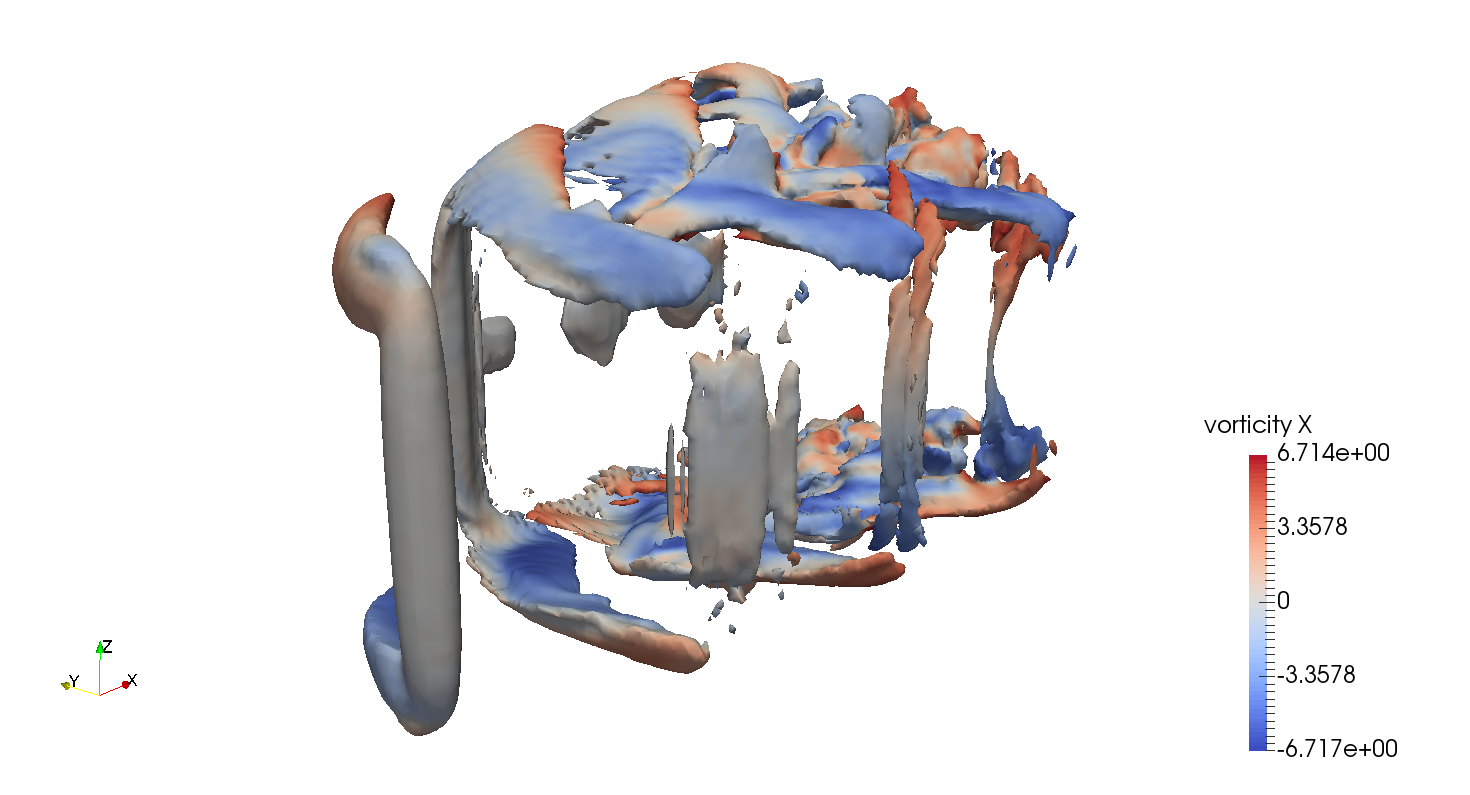
\includegraphics[width=0.8\textwidth]{RVAT-ALM-LES_vorticity-snapshot}

    \caption{Snapshot of vorticity isosurfaces (colored by their streamwise
        component) at $t=6$ s for the UNH-RVAT LES case.}

    \label{RVAT-ALM-LES-vorticity}
\end{figure}

The near-wake's mean velocity field at $x/D=1$ is shown in
Figure~\ref{RVAT-ALM-LES-vorticity}. Compared with the RANS ALM results, the LES
looks much more like the blade-resolved and experimental results, showing the
clockwise and counterclockwise mean swirling motion on the $-y$ and $+y$ sides
of the rotor, respectively.

\begin{figure}
    \centering

    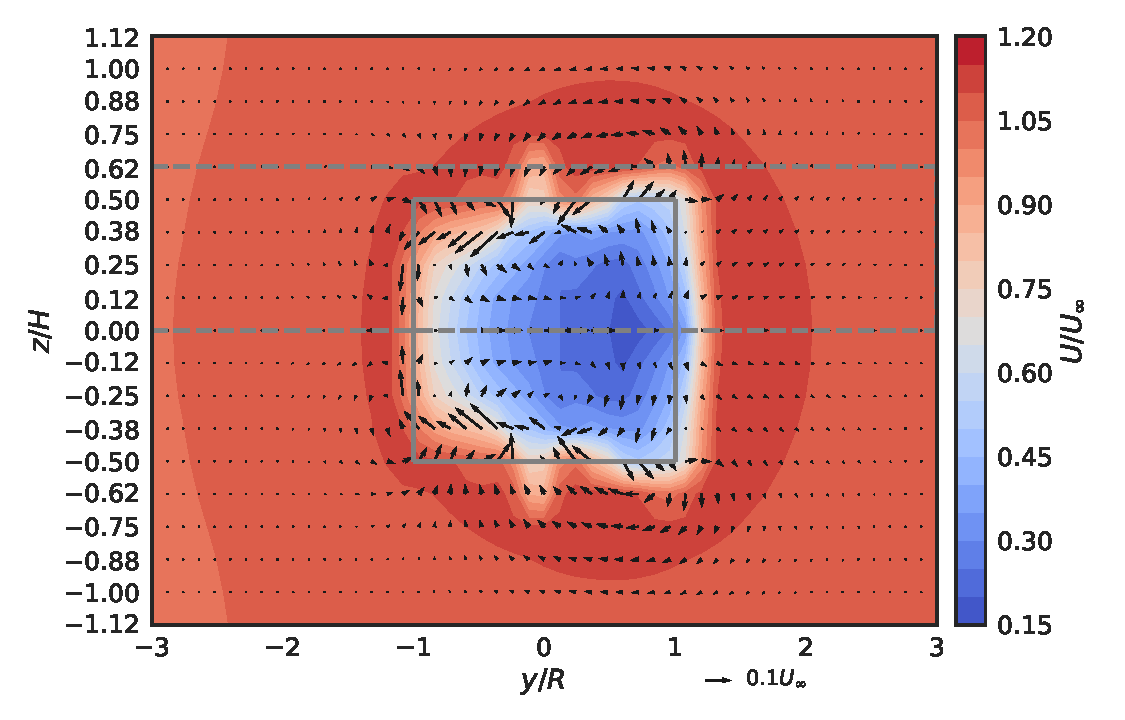
\includegraphics[width=0.75\textwidth]{RVAT-ALM-LES_meancontquiv}

    \caption{Mean velocity field in the UNH-RVAT near-wake at $x/D=1$ computed
        with the Smagorinsky LES model.}

    \label{fig:RVAT-ALM-LES-meancontquiv}
\end{figure}

Contours of turbulence kinetic energy sampled at $x/D=1$ from the large eddy
simulation are plotted in Figure~\ref{fig:RVAT-ALM-LES-kcont}. Compared with
RANS, LES is more able to predict the turbulence generated by the blade tip
vortex shedding and dynamic stall effects, though the overall level of
unsteadiness generated was much lower, especially on the $+y$ side of the rotor.
This is likely a consequence of the SGS modeling, where the vortical structures
generated by the blades remain stable further downstream. Similar effects were
seen in \cite{Martinez-Tossas2015a, Shamsoddin2014}, where higher levels of the
Smagorinsky coefficient delayed vortex breakdown and subsequent higher levels of
turbulence. Figure~\ref{RVAT-ALM-LES-vorticity} shows evidence of these effects,
where the blade bound and tip vortices are still relatively coherent at $x/D=1$.

\begin{figure}
    \centering

    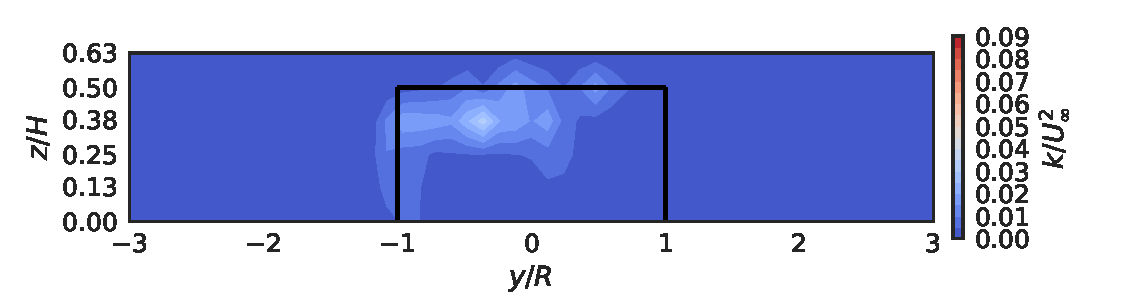
\includegraphics[width=0.7\textwidth]{RVAT-ALM-LES_kcont}

    \caption{Turbulence kinetic energy in the UNH-RVAT near-wake at $x/D=1$
        computed with the Smagorinsky LES model.}

    \label{fig:RVAT-ALM-LES-kcont}
\end{figure}

Mean velocity profiles at the turbine center plane, plotted in
Figure~\ref{fig:RVAT-ALM-LES-profiles}, were predicted more accurately using LES
versus RANS, and rival those of the 3-D blade-resolved models. However,
turbulence kinetic energy profiles did not match as closely with experiments.
Though the qualitative shape was resolved better than that by the RANS ALM
simulation, notably the asymmetric peaks around $y/R = \pm 1$, the turbulence
generated in the large eddy simulation was approximately an order of magnitude
too low. Once again this was probably a result of the subgrid-scale modeling and
its effect on the stability of vortex structures.

\begin{figure}
    \centering

    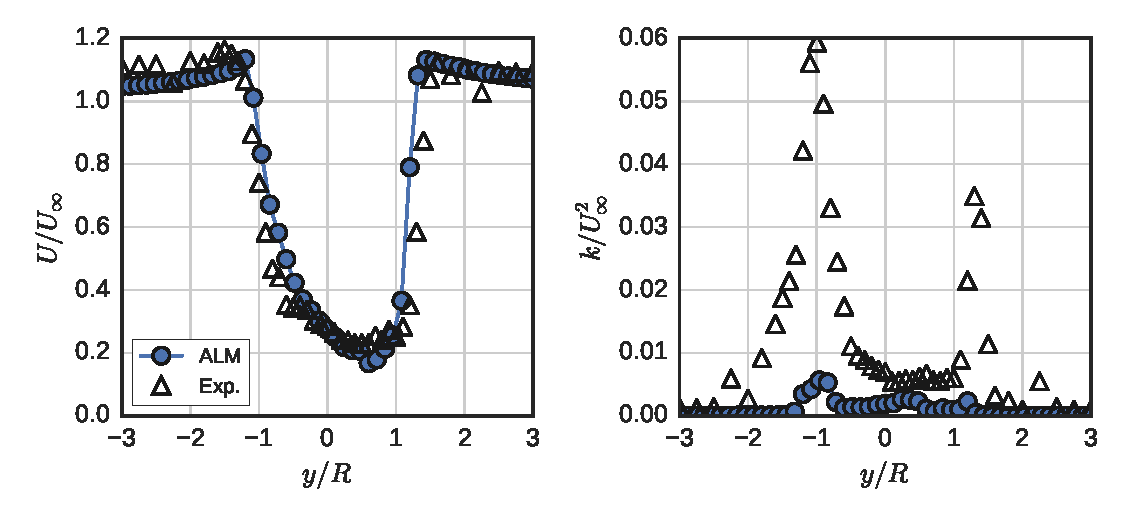
\includegraphics[width=0.7\textwidth]{RVAT-ALM-LES_wake-profiles}

    \caption{Mean velocity profiles in the UNH-RVAT near-wake at $x/D=1$ and
        $z/H=0$ computed with the Smagorinsky LES model.}

    \label{fig:RVAT-ALM-LES-profiles}
\end{figure}

The planar weighted sums of streamwise momentum recovery terms were computed in
the same way as for the RANS cases with the exception of the turbulent transport
term, which for the LES was computed from the $x$-components of the divergence
of the resolved and SGS Reynolds stress tensors:
\begin{equation}
    \text{Turb. trans.} = - \left( \frac{\partial}{\partial x_j}
    \overline{u^\prime_x u^\prime_j}
    + \frac{\partial}{\partial x_j} R_{xj}
    \right),
\end{equation}
where $u$ indicates the resolved or filtered velocity, and $R$ is the
subgrid-scale Reynolds stress.

Transport term weighted sums computed from the LES results are shown in
Figure~\ref{fig:RVAT-ALM-LES-recovery}. Unlike the RANS ALM cases, the
cross-stream advection contributions are negative, as they are in the experiment
and blade-resolved CFD models. The vertical advection term is positive as
expected, though smaller than in other cases. Interestingly, the turbulent
transport is negative in the LES, meaning the combined effects of the resolved
and SGS stressed are transferring momentum out of the wake. The low turbulent
transport appears to be partially balanced by higher levels of viscous
diffusion---about an order of magnitude larger than the 3-D blade-resolved RANS
models and experiments. These discrepancies highlight the difficulty of
predicting the near-wake dynamics, the importance of the SGS model in LES, and
the need for data further downstream to test and refine predictions for wake
evolution. For example, setting the Smagorinsky coefficient higher may induce
vortex breakdown earlier, which would raise the turbulence levels significantly.

\begin{figure}
    \centering

    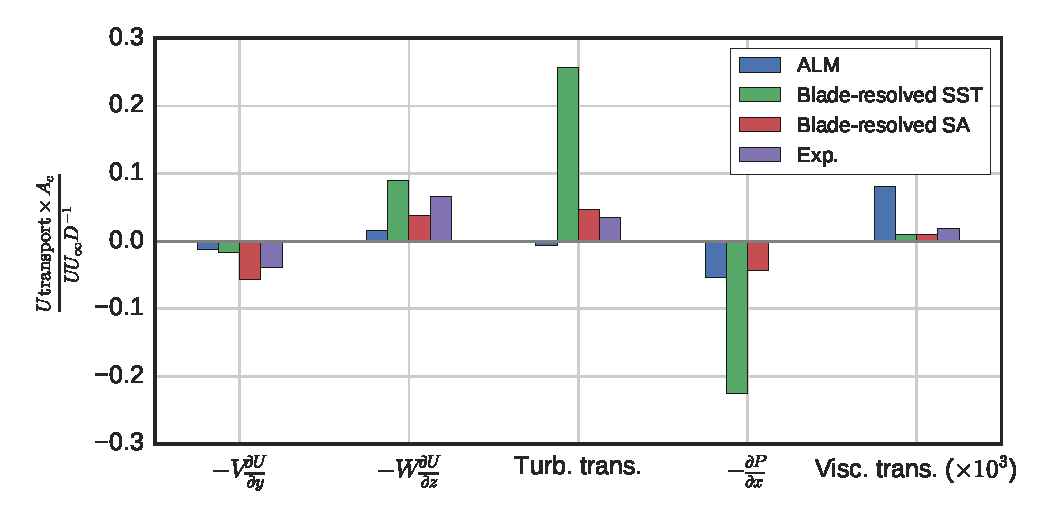
\includegraphics[width=0.7\textwidth]{RVAT-ALM-LES_recovery-bar-chart}

    \caption{Weighted average momentum recovery terms at $x/D=1$ for the RVAT
        ALM LES using the Smagorinsky SGS model.}

    \label{fig:RVAT-ALM-LES-recovery}
\end{figure}


\section{Conclusions}

An actuator line model for cross-flow turbines, including a Leishman--Beddoes
type dynamic stall model, flow curvature, added mass, and lifting-line based end
effects corrections, was developed and validated against experimental datasets
acquired for high and medium-low solidity rotors at scales where the performance
and near-wake dynamics were essentially Reynolds number independent. When
coupled to a $k$--$\epsilon$ RANS solver ALM simulations took $O(0.1)$ CPU hours
per second of simulated time, while when coupled with a Smagorinsky LES model
the computing time was $O(10)$ hours per second, which represent a four and two
order of magnitude decrease in computational expense versus 3-D blade-resolved
RANS, respectively.

The RANS ALM predicted the UNH-RVAT performance well at tip speed ratios up to
and including that of max power coefficient. The RM2 power coefficient on the
other hand was underpredicted at lower $\lambda$. Both models overestimated
$C_P$ at the highest tip speed ratios, which has been observed in other
simulations using Leishman--Beddoes type dynamic stall models. Possible
explanations include underestimation of added mass effects or blade--strut
connection corner drag, incorrect time constants in the LB DS model, and/or
inaccuracy due to the virtual camber effect. In the present flow curvature
model, the angle of attack is corrected, but the foil coefficient data is not
transformed, meaning the LB DS separation point curve fit parameters are equal
for both positive and negative angles of attack. A foil data transformation
algorithm based on virtual camber should be investigated for future improvement
of the ALM.

The RANS ALM cases were able to match some important qualitative near-wake flow
features, e.g., the mean vertical advection velocity towards the mid-rotor
plane. However, the mean flow structure and turbulence generation due to blade
tip and dynamic stall vortex shedding shows some discrepancy with experimental
and blade-resolved CFD. Extensions to the ALM to deal with these shortcomings
should be developed, e.g., a turbulence injection model as employed by James et
al. \cite{James2010} or a model that will ``turn'' the ALM body force vectors to
approach the effects of leading and trailing edge vortex shedding during dynamic
stall.

The UNH-RVAT was simulated with the ALM embedded within a typical Smagorinsky
LES, which thanks to its lower diffusion and/or dissipation was able to more
accurately capture the large scale vortical flow structures shed by the rotor
blades. Turbulence generated by the blade tip vortex shedding and dynamic stall
region of the blade path was better resolved, but overall lower levels of
turbulence were predicted, which is likely a consequence of the subgrid-scale
model's influence on the stability of shed vortices. This effect was also
apparent in the negative predictions of turbulent transport on the streamwise
momentum recovery. Therefore, subgrid-scale modeling should be investigated
further before applying the ALM LES to array analyses.

The ALM provides a more physical flow description compared to momentum and
potential flow vortex models, at a reasonable cost. The ALM also drastically
reduces computational effort compared to blade-resolved CFD, while maintaining
the unsteadiness of the wake not resolved by a conventional actuator disk.
Furthermore, its implementation within finite volume CFD provides a convenient
way to study turbine array siting, since effects like terrain and buildings can
be included, as can no-slip boundary conditions and boundary layer inflow
profiles. Since the turbinesFoam library developed here uses OpenFOAM's modular
\texttt{fvOptions} framework, the ALM body force term can be added as-is to
compressible or multiphase solvers, for exploring more complicated physics.
These features would be difficult or impossible to implement in a momentum or
vortex models.

Ultimately, the ALM retains some of the disadvantages of other blade element
methods, but is a the next logical step bridging the gap between low- and
high-fidelity flow modeling, and has been shown to be a method worthy of further
advancement. The prospect of using ALM simulations to drive down computational
cost of RANS by roughly four orders of magnitude---enabling 3-D unsteady
Navier--Stokes simulations to be performed on a typical PC---itself justifies
further development.

At contemporary levels of computing power, the ALM is a useful tool for studying
individual turbines when HPC is not feasible---requiring similar resources as
2-D blade-resolved RANS, but with improved performance predictions. Furthermore,
if arrays of CFTs advance to commercial scale, the ALM combined with LES
represents one of the highest fidelity tools available, and will improve as
turbulence modeling improves. It is therefore expected that this tool will prove
valuable for both the engineering and research of wind and MHK turbines.


\section{Future work}

The actuator line model shows great potential for use in cross-flow turbine
engineering, and this study has inspired many avenues for its improvement.

Firstly, since the fundamental premise of the ALM relies on accurate static foil
coefficient data, it is crucial that more be measured and published openly, to
allow the exploration of new rotor designs with various profiles. There is some
doubt regarding the veracity of the Sheldahl and Klimas NACA foil data
\cite{Bedon2014}. However, competing datasets at large laboratory scale Reynolds
numbers are rare, even for the standard symmetrical foils. CFD may play a role
in generating new data, but models must be rigorously validated, given the
difficulty in predicting stall and its importance on CFT blade loading.

Profile coefficient databases could be expanded to include more dimensions, or
independent variables. For example, since the ALM will almost always involve
turbulence modeling, the effects of local turbulence levels on foil coefficient
data could be included, since stall delay could affect loading significantly,
especially for a cross-flow turbine.

Dynamic stall model empirical constants should be further investigated for their
optimal values within the cross-flow turbine context. Though the
Leishman--Beddoes type models are formulated in terms of a nondimensional time,
there may be a dependence of the various time constants on the pitch rate, as
indicated by the improvement in predictions for the RM2 at optimal tip speed
ratio when using a higher angle of attack lag time constant. Machine learning
techniques could be employed to ``train'' the constants (and/or their
$\lambda$-dependence) to one turbine's power curve, and they could be validated
against the other turbine's data. A more data-intensive alternative could be to
develop dynamic cyclic profile coefficient databases---either experimentally or
numerically---for many reduced frequencies, though this would be a difficult
task, even for a single profile.

Flow curvature corrections should be examined in more detail, and it may be
beneficial to develop models to transform entire foil datasets to match their
virtual camber, as suggested by Migliore et al.~\cite{Migliore1980}. It
also may be advantageous to implement a complementary model to adjust the
direction of the resultant force vector to more accurately generate the blade's
shed vorticity.

Rotor angular speed control via generator models could be included to test the
effectiveness of various control schemes, e.g., sinusoidal $\lambda$ set points,
which have been shown in some cases to improve mean power coefficient
\cite{Strom2015}. Free stream velocity sampling could be implemented to
determine the optimal location for sensing reference velocity used to compute
tip speed ratio and power coefficient, which can become difficult in sheared or
otherwise nonuniform flows \cite{Forbush2015}.

Since turbinesFoam is compatible with OpenFOAM's volume of fluid (VOF)
multiphase flow solver interFoam, the ALM's effectiveness should be assessed for
predicting the generation and interaction of turbines with surface waves. Tow
tank experiments could be performed with a wave gauge to measure and validate
the free surface disturbance, which could be key to predicting the effects of
placing turbines in channels at high blockage ratio.

Possibly most importantly, the ALM should be validated with far-wake velocity
measurements and/or performance data from two CFTs operating in proximity of
each other. Next, the ALM should be evaluated for its use in modeling CFT arrays
using both RANS and LES. If either can successfully postdict experimentally
measured performance of closely-spaced physical model CFTs, they should then be
coupled with optimization algorithms to automatically explore the design space,
and ultimately drive down the cost of energy.


\acks The authors would like to acknowledge funding through a National Science
Foundation CAREER award (principal investigator Martin Wosnik, NSF 1150797,
Energy for Sustainability, program manager Gregory L. Rorrer). This work has
been carried out as part of author P. Bachant's PhD research at the University
of New Hampshire.

\bibliographystyle{wileyj}
\bibliography{library}
\end{document}
